\documentclass{beamer}

%% \documentclass[handout]{beamer}
%% % use this with the [handout] option to create handouts for the audience
%% \usepackage{pgfpages}
%% \pgfpagesuselayout{2 on 1}[a4paper,border shrink=5mm]

\mode<presentation>
{
  \usetheme{Diku}
% set this to your preferences:
  \setbeamercovered{invisible}
%  \setbeamercovered{transparent}
}

\usepackage{graphicx}
\usepackage{epic}

\usepackage{amsmath}
\usepackage{amssymb}
\usepackage{amsthm}

\newcommand{\basetop}[1]{\vtop{\vskip-1ex\hbox{#1}}}
\newcommand{\source}[1]{\let\thefootnote\relax\footnotetext{\scriptsize\textcolor{kugray1}{Source: #1}}}

% for coloured code citation in text:
\usepackage{fancyvrb}

%%%%%%%%%%%%%%%%%%%%%%%%%%%%%%%%%
%%%%%    code sections   %%%%%%%%
%%%%%%%%%%%%%%%%%%%%%%%%%%%%%%%%%

% code highlighting commands in own block
\DefineVerbatimEnvironment{code}{Verbatim}{fontsize=\scriptsize}
\DefineVerbatimEnvironment{icode}{Verbatim}{fontsize=\scriptsize}

% Fancy code with color commands:
\DefineVerbatimEnvironment{colorcode}%
        {Verbatim}{fontsize=\scriptsize,commandchars=\\\{\}}

%%%%%%%%%%%%%%%%%%%%%%%%%%%%%%%%%%
%%%%%    some coloring    %%%%%%%%

\definecolor{Red}{RGB}{220,50,10}
\definecolor{Blue}{RGB}{0,51,102}
\definecolor{Yellow}{RGB}{102,51,0}
\definecolor{Orange}{RGB}{178,36,36}
\definecolor{Grey}{RGB}{180,180,180}
\definecolor{Green}{RGB}{20,120,20}
\definecolor{Purple}{RGB}{160,50,100}
\newcommand{\red}[1]{\textcolor{Red}{{#1}}}
\newcommand{\blue}[1]{\textcolor{Blue}{{#1}}}
\newcommand{\yellow}[1]{\textcolor{Yellow}{{#1}}}
\newcommand{\orange}[1]{\textcolor{Orange}{{#1}}}
\newcommand{\grey}[1]{\textcolor{Grey}{{#1}}}
\newcommand{\green}[1]{\textcolor{Green}{{#1}}}
\newcommand{\purple}[1]{\textcolor{Purple}{{#1}}}




% use "DIKU green" from our color theme for \emph
\renewcommand{\emph}[1]{\textcolor{structure}{#1}}
% use some not-too-bright red for an \emp command
\definecolor{DikuRed}{RGB}{130,50,32}
\newcommand{\emp}[1]{\textcolor{DikuRed}{ #1}}
\definecolor{CosGreen}{RGB}{10,100,70}
\newcommand{\emphh}[1]{\textcolor{CosGreen}{ #1}}
\definecolor{CosBlue}{RGB}{55,111,122}
\newcommand{\emphb}[1]{\textcolor{CosBlue}{ #1}}
\definecolor{CosRed}{RGB}{253,1,1}
\newcommand{\empr}[1]{\textcolor{CosRed}{ #1}}

\newcommand{\mymath}[1]{$ #1 $}
\newcommand{\myindx}[1]{_{#1}}
\newcommand{\myindu}[1]{^{#1}}

\newcommand{\Fasto}{\textsc{Fasto}\xspace}


%%%%%%%%%%%%%%%%%%%%

\title[Intro]{Introduction: Hardware Trends\\and Vector Machines}

\author[C.~Oancea]{Cosmin E. Oancea {\tt cosmin.oancea@diku.dk}}

\institute{Department of Computer Science (DIKU)\\University of Copenhagen}


\date[Sept 2014]{September 2014 PMPH Lecture Notes}


\begin{document}

\titleslide


%%%%%%%%%%%%%%%%%%%%%%%%%%%%%%%%%%%%%%%%%%%%%%%%%%%%%%%%%%%%%%%%%%%%%%
%%%%%%%%%%%%%%%%%%%%%%%%%%%%%%%%%%%%%%%%%%%%%%%%%%%%%%%%%%%%%%%%%%%%%%
%%%%%%%%%%%%%%%%%%%%%%%%%%%%%%%%%%%%%%%%%%%%%%%%%%%%%%%%%%%%%%%%%%%%%%
\begin{frame}[fragile]
	\tableofcontents
\end{frame}

%%%%%%%%%%%%%%%%%%%%%%%%%%%%%%%%%%%%%%%%%%%%%%%%%%%
%%%%%%%%%%%%%%%%%%%%%%%%%%%%%%%%%%%%%%%%%%%%%%%%%%%
%%%%%%%%%%%%%%%%%%%%%%%%%%%%%%%%%%%%%%%%%%%%%%%%%%%

%\section{Scalable Shared Memory Systems}

\section{Introduction$^{\mbox{\bf 2}}$}

\subsection{Brief History}

\begin{frame}[fragile,t]
\frametitle{Introduction$^{\mbox{\bf 2}}$}

\begin{itemize}
    \item Past $>$ 20 years \emph{Information Revolution}:\\
        Explosive growth of semiconductor integration + Internet.\bigskip

    \item Moore's Low 1960s: 
    \begin{itemize}
        \item computing power doubles every 19-24 months 
        \item \emph{system cost effectiveness = {\tt performance/cost} 
                grows exp}.
        \item \alert{CMOS endpoint is near}: miniaturization reaches its limits
                (complementary metal-oxide semiconductor).
    \end  {itemize}\bigskip

    \item Improved Chip Design:
    \begin{itemize}
        \item each new process generation $\Rightarrow$ higher clock rates 
        \item logic switching speed \& amount of on-chip logic increase ($\uparrow$)
        \item better circuit design \& deep pipelines $\Rightarrow$ 
                fewer gate delays / stage
        \item $\uparrow$ on-chip resources $\Rightarrow$ $\uparrow$ throughput by 
                parallelism at all stages. 
    \end  {itemize}\bigskip

    \item \emp{Computer Arch 1970s: How to Best Use the ever-increasing ($\uparrow$) 
            Wealth of Resources?}

\end{itemize}

\end{frame}

\begin{frame}[fragile,t]
\frametitle{Brief History}

\begin{itemize}
        \item \emph{ICPP, ISCA 1980/90s: parallel architectures popular topic.}\\
              Demise of SingleCPU System: inevitable \& fast approaching.\bigskip

        \item \alert{Whatever happened? Mid90 Killer-Micro:}
        \begin{itemize}
            \item The rapid increase ($\uparrow$) transistor density $\Rightarrow$\\
            \item path of least resistance: ever-increasing speed of SingleCPU
            \item Complex Out-Of-Order (OoO) processors: 100s instructions/cycle.
            \item Commercial arena: multiprocessors just an uniprocessor extension.
        \end  {itemize}\bigskip

        \item \alert{What Changed?} Multiprocessors Trend: Academia \& Industry:
        \begin{itemize}
            \item \emp{power complexity}
            \item \emp{Memory WALL}: $\uparrow$ performance gap between processor \& memory 
        \end  {itemize}\bigskip

       \item \emph{All Future Architectures adopt some form of massive parallelism!}
\end{itemize}

\end{frame}


\subsection{Computer Architecture Definition}

\begin{frame}[fragile,t]
\frametitle{What used to Be Computer Architecture?}

\begin{columns}\hspace{-8ex}
\column{0.6\textwidth}
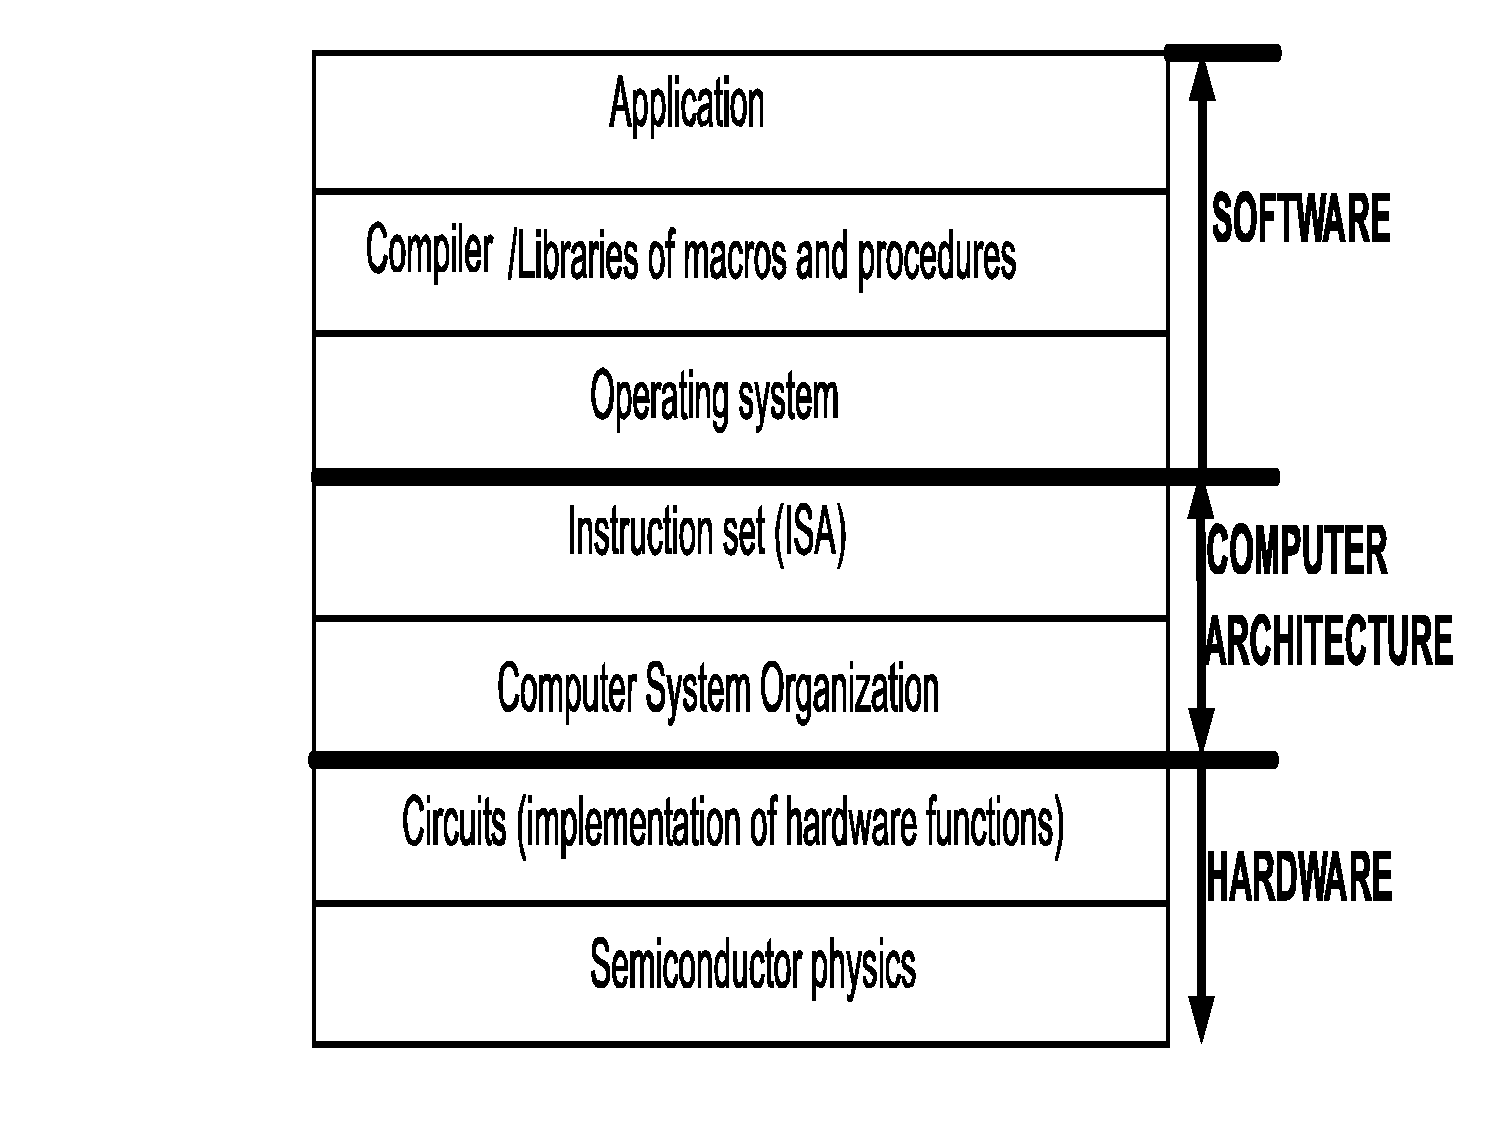
\includegraphics[width=44ex]{Ch1Figs/SysOrg}
\column{0.65\textwidth}\vspace{-3ex}
\begin{itemize}
    \item Multi-Layered: focus competences.
    \item Each layer uses the ones below it.
    \item \emp{Application} C++/Java/SML/Haskell.
    \item \emp{Compiler}: machine code + OpSys calls.
    \item \emp{OpSys}: extends hardware funct \&
              orchestrates resource sharing among multiple users.
    \item \emp{ISA \& Computer Organization}: 
            software-hardware interface. 
\end{itemize}
\end{columns}

\emp{Old Definition} ISA -- critical role in the success of computer industry:
\begin{itemize}
    \item Early on, used to be the hallmark of system design $\Rightarrow$
    \item Non-Portable Software \& No Compiler at that time
    \item 1960s IBM System360 ISA guarantees backward compatibility $\Rightarrow$
    \item Strategy endured test of time \& Behemoth company today
\end{itemize}
\end{frame}



\begin{frame}[fragile,t]
\frametitle{What Is Computer Architecture Today?}

\begin{columns}
\column{0.59\textwidth}
\hspace{-6ex}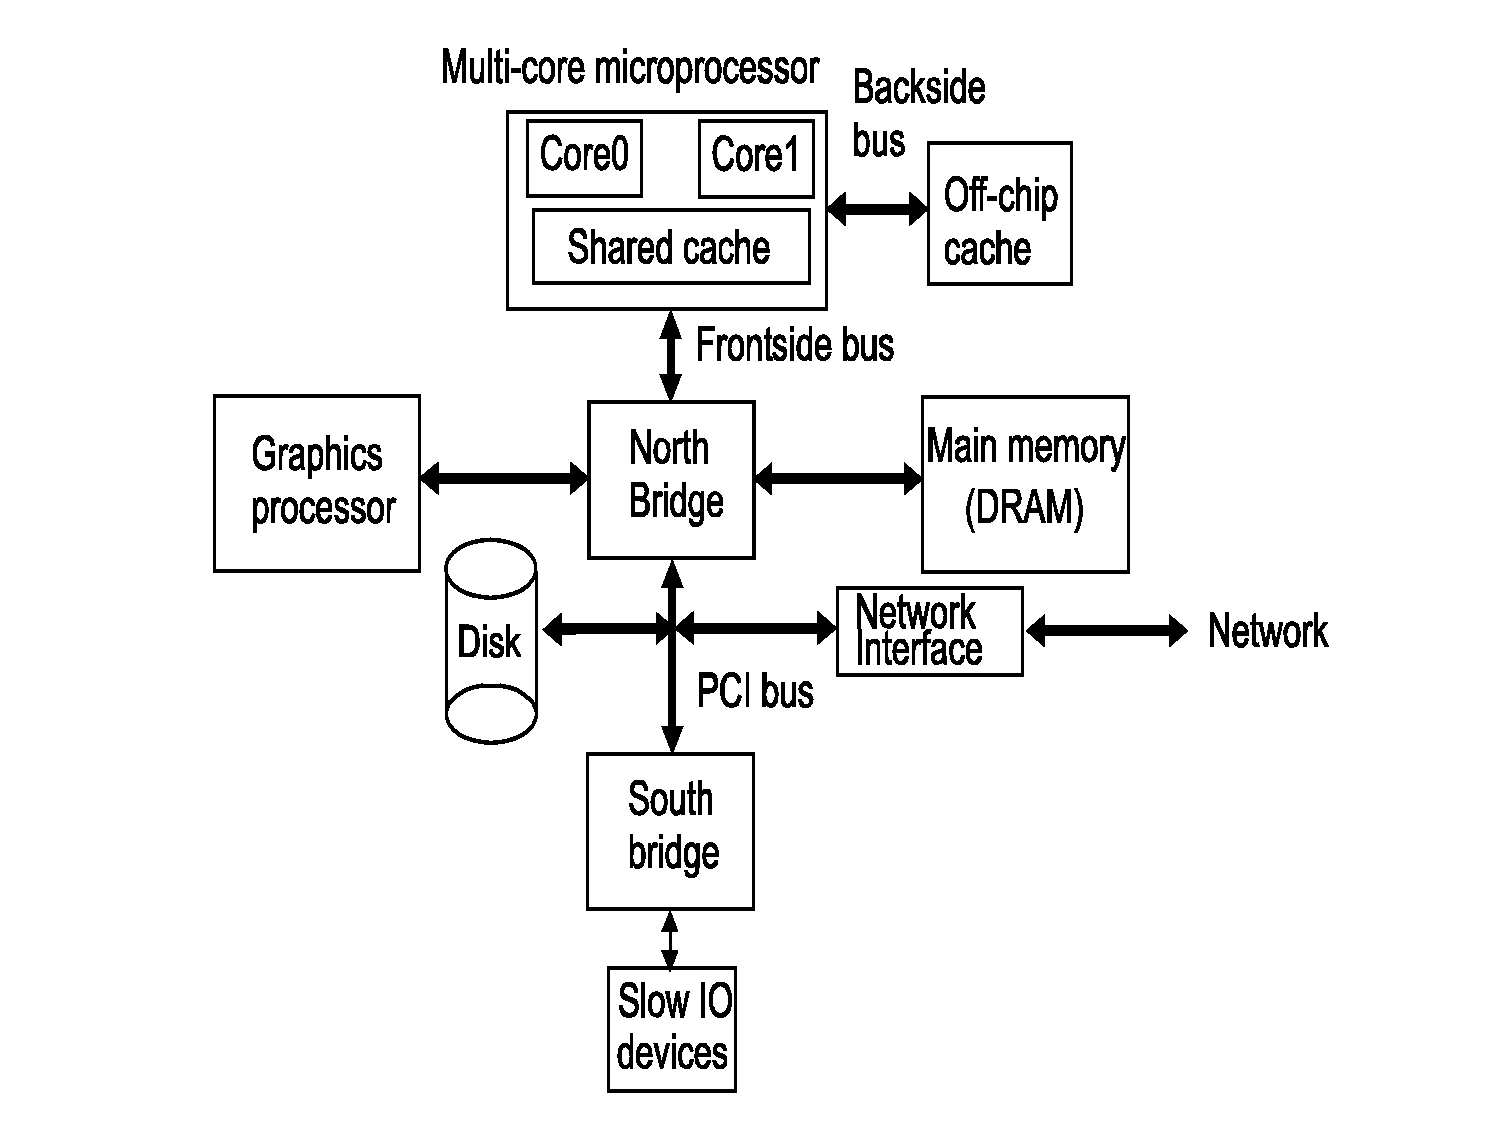
\includegraphics[width=44ex]{Ch1Figs/SimpleCPU}

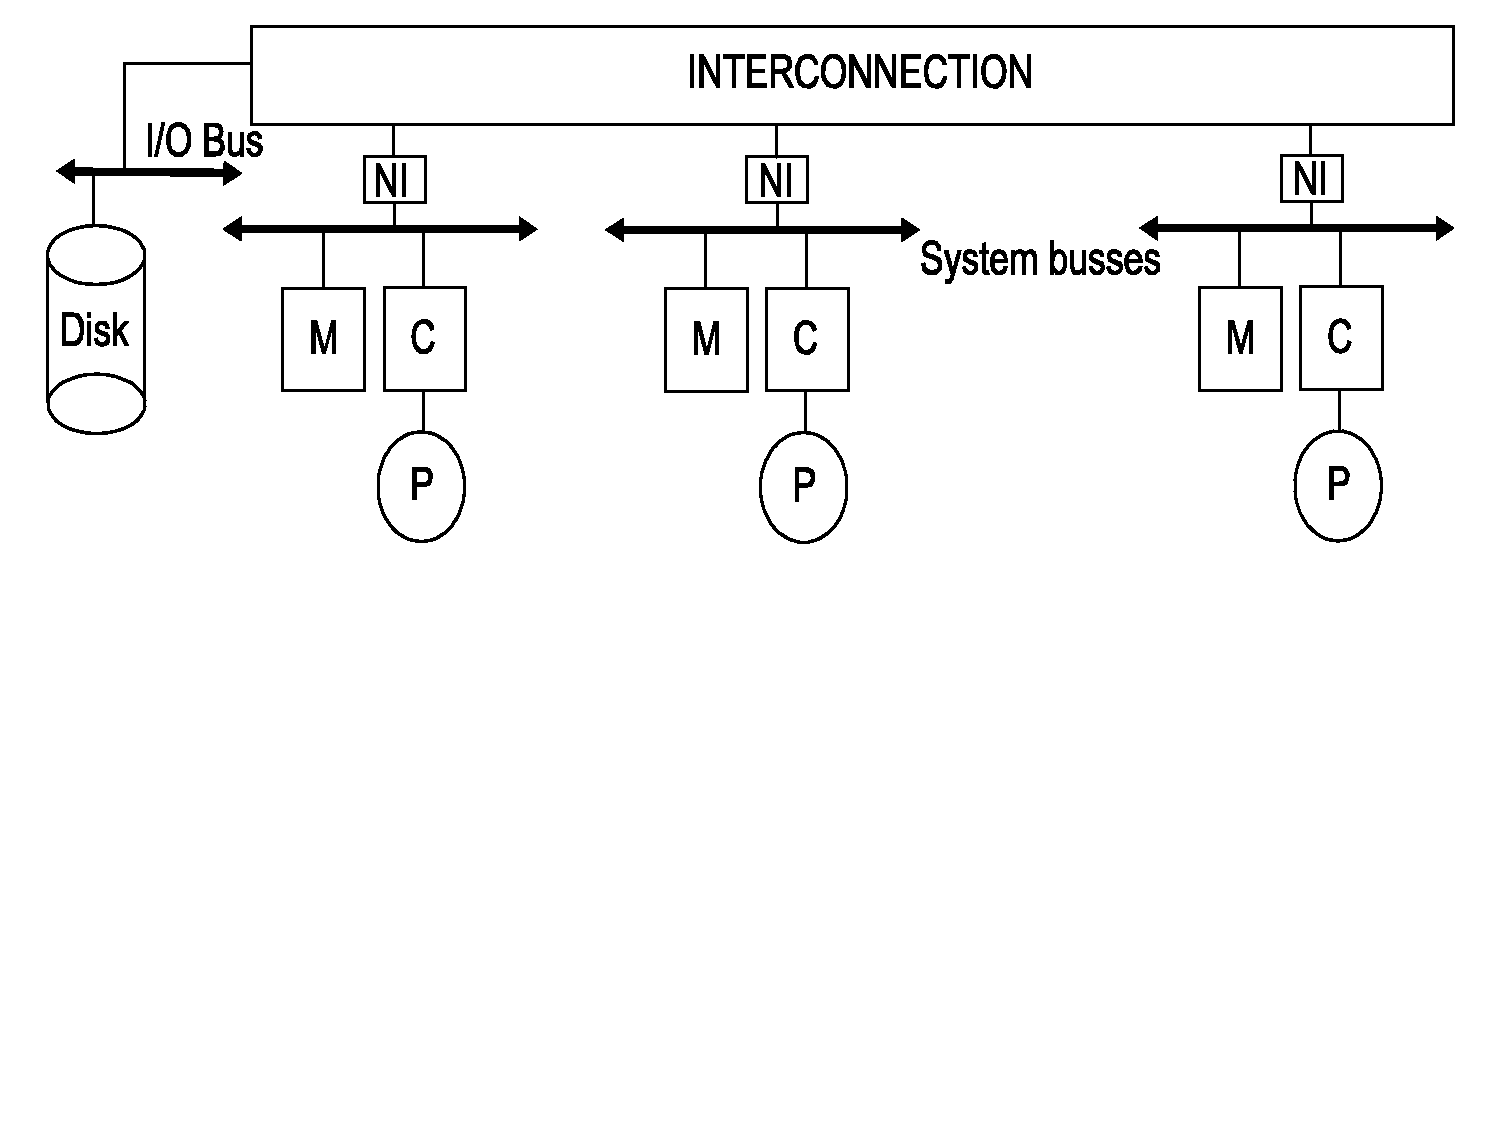
\includegraphics[width=39ex]{Ch1Figs/SimpleInterconnect}
\column{0.55\textwidth}\vspace{-17ex}
\begin{itemize}
    \item \emp{Much Broader Definition}: how best to build the computer 
            (includes ISA, but focus changed on organization).\medskip

    \item North Bridge: sys bus connects cores to memory \& IO devs.
    \item PCI bus: IO bus connecting North Bridge to high-speed IO 
            to disk, network \& slower dev\medskip

    \item $\leftarrow$ Generic Multiprocessor with Distributed Memory\medskip

    \item \alert{Parallel Sys Main Components:
                (1) Processor, (2) Memory Hierarchy and 
                (3) Interconnection}
\end{itemize}
\end{columns}

\end{frame}



\begin{frame}[fragile,t]
\frametitle{Software-Hardware Synergy \& Biggest Challenge}
\medskip
\begin{columns}
\column{0.33\textwidth}
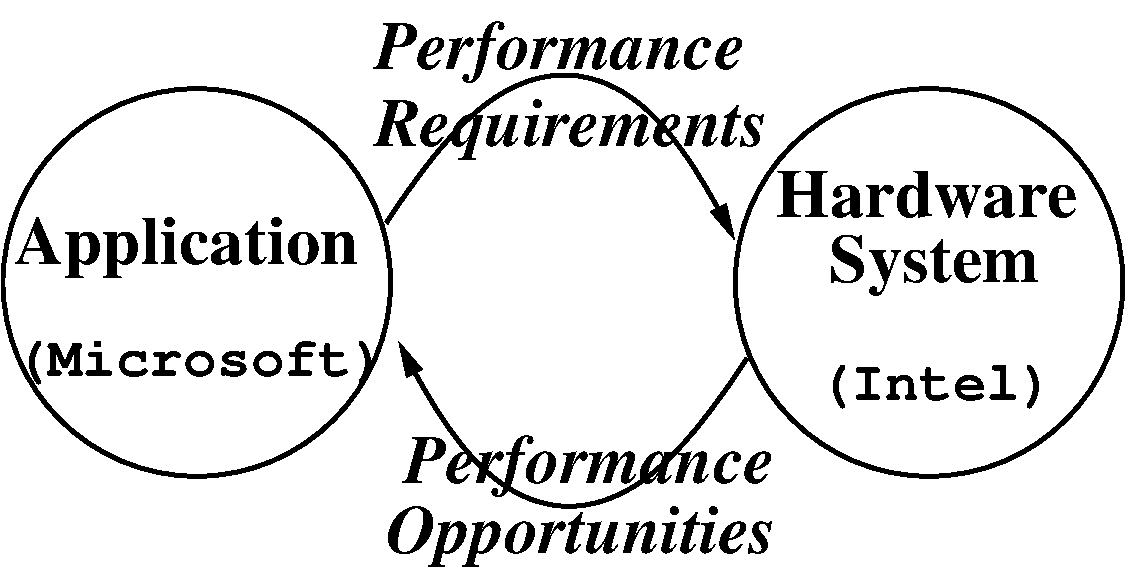
\includegraphics[width=29ex]{Ch1Figs/Synergy}
\column{0.63\textwidth}\vspace{-3ex}
\begin{itemize}
    \item Computer Architect Role:
    \item \emp{design trade-offs across HW/SW interf to meet functional 
            \& performance requirements within cost constraints.}
\end{itemize}
\end{columns}
\medskip

\begin{itemize}
    \item software: flexible approach to simplifying hardware, 
            e.g., TLB exceptions, FP ops,
    \item hardware faster $\Rightarrow$ world of tradeoff in between 
    \item guided by the common case $\Rightarrow$ trends are important.\bigskip

    \item \emp{Important Juncture:} 
        \begin{itemize}
            \item \emph{Higher performance requires Parallel Hardware}
            \item \alert{Biggest Challenge: 
                    develop Effective Massively Parallel Software!}
        \end  {itemize}
\end{itemize}
\end{frame}


\subsection{Course Organization}
\begin{frame}
\frametitle{Course Organization}

\begin{tabular}{lccccc}
W  & HARDWARE  & & SOFTWARE     & & LAB/CUDA \\\hline\hline
1 & \alert{Trends}         &                         & \emp{List HOM}     & & \emph{Intro \& Simple}\\
  & \alert{Vector Machine} & \emph{$\longleftarrow$} & \emp{(Map-Reduce)} & & \emph{Map Programming}\\\hline
%
2 & In Order & $\longrightarrow$ & VLIW Instr   & & Scan \&\\
  & Processor& $\longleftarrow$ & Scheduling   & & Reduce \\\hline
%
3 & Cache     & & Reasoning About     & & Sparse Vect\\
  & Coherence & & Parallelism   & & Matrix Mult\\\hline
%
4 & Interconnection & & Case Studies \&   & & Transpose \& Matrix\\
  & Networks        & & Optimizations   & & Matrix Mult\\\hline
%
5 & Memory      & & Optimising   & & Sorting \& Profiling \& \\
  & Consistency & & Locality     & & Mem Optimizations \\\hline
%
6 & OoO, Spec   & & Thread-Level   & & Project \\
  & Processor   & & Speculation    & & Work    \\\hline

%\framebox{Processor}       & & \framebox{Low-Level\\Optimizations}        & & \framebox{CUDA: Scan\\Reduce}\\
%$\downarrow$ && $\uparrow$ \\
%\framebox{\red Intermediate code generation} &$\longrightarrow$ & Intermediate code
\end{tabular}
\medskip
%\alert{Keywords: Reasoning, Tradeoffs, Common Case, }

Three narative threads: the path to complex \& good design: 
\begin{itemize}
    \item \emp{Design Space} tradeoffs, constraints, common case, trends.
    \item \emp{Reasoning}: from simple to complex, \emp{Applying Concepts}.
\end  {itemize}
\end{frame}



%%%%%%%%%%%%%%%%%%%%%%%%%%%%%%%%%%%%%%%%%%%%%

\section{Trends of Critical Components of a Parallel System}

\begin{frame}[fragile]
	\tableofcontents[currentsection]
\end{frame}

\subsection{Processor}

\begin{frame}[fragile,t]
\frametitle{Abstractions}
\medskip

\begin{itemize}
%    \item[Program] set of statements performing computational steps.
%    \item[Process/Thread] embeds the execution of the computation.
    \item A \emp{program} is to a \emp{process/thread} 
            what a recipe is for cooking.\smallskip

    \item \emp{Processor (core)}: hardware entity capable of
            sequencing \& executing thread's instructions.\smallskip

    \item \emp{MT Cores} multiple threads, each 
            running in its thread context.\smallskip

    \item \emp{Multiprocessor:} set of processors connected to execute a workload
        \begin{itemize}
            \item mass produced, off-the-shelf, each several cores \& levels of cache
            \item trend towards migrating system functions on the chip:\\
                    memory controllers, external cache directories, network interface
        \end  {itemize}
\end{itemize}

%\begin{columns}
%\column{0.33\textwidth}
%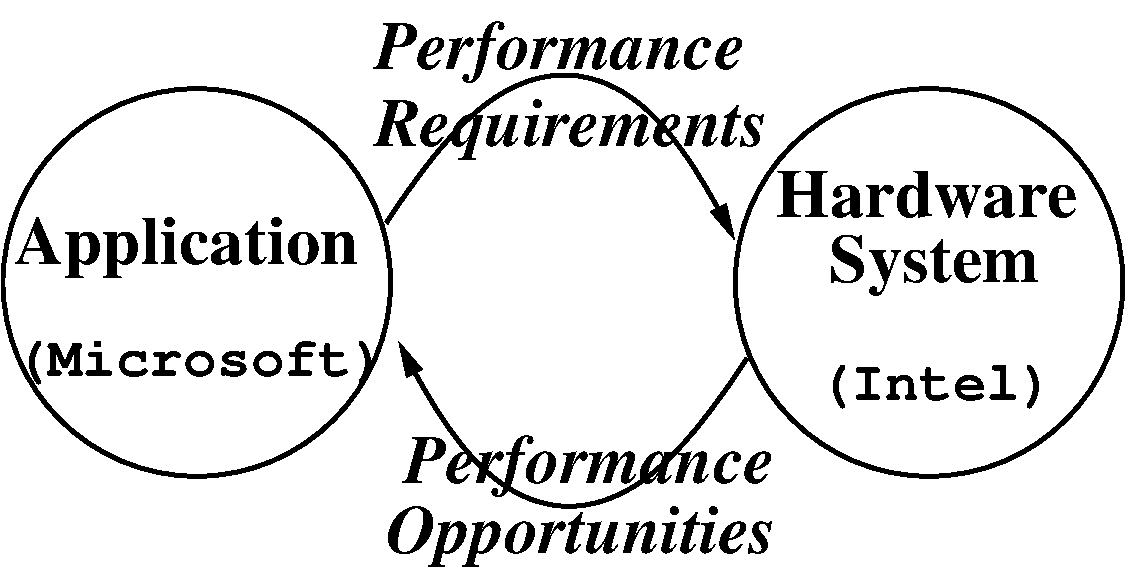
\includegraphics[width=29ex]{Ch1Figs/Synergy}
%\column{0.63\textwidth}\vspace{-3ex}
%\begin{itemize}
%    \item Computer Architect Role:
%    \item \emp{design trade-offs across HW/SW interf to meet functional 
%            \& performance requirements within cost constraints.}
%\end{itemize}
%\end{columns}

\end{frame}


\begin{frame}[fragile,t]
\frametitle{Processor: Clock Frequency/Rate}

Historically the clock rate (at which instr are executed) has increased 
exponentially (1990-2004).

\begin{columns}
\column{0.65\textwidth}
\hspace{-5ex}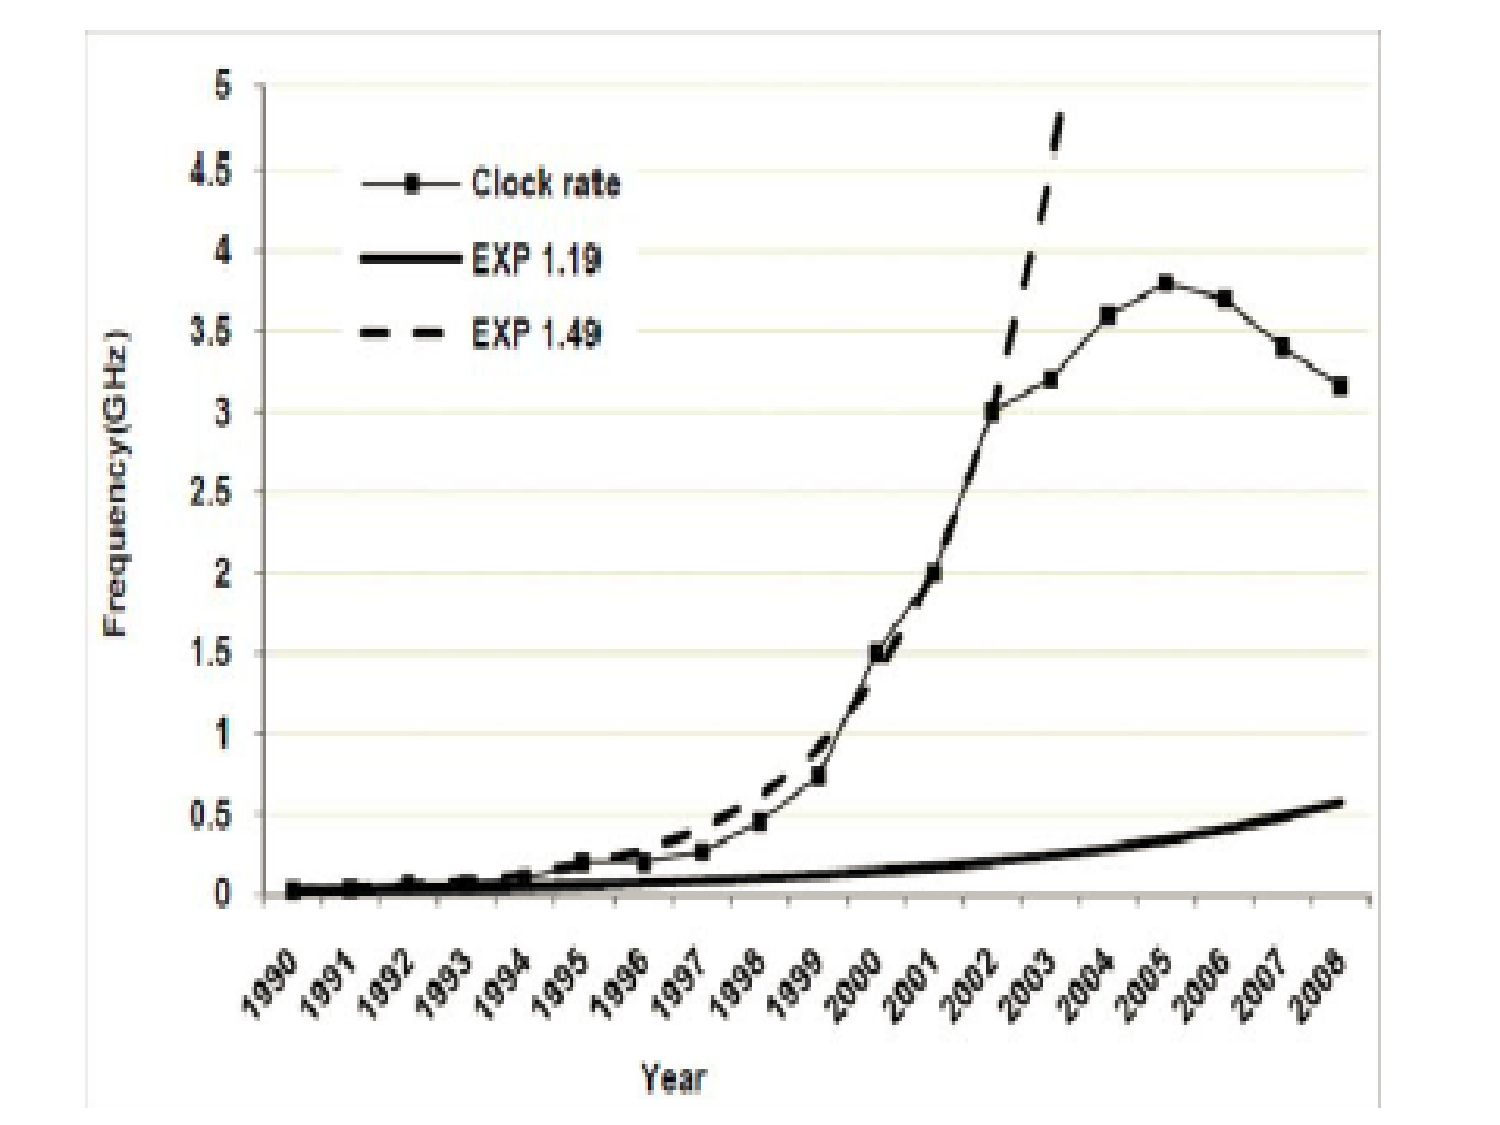
\includegraphics[width=52ex]{Ch1Figs/FreqGraph}\pause
\column{0.48\textwidth}\vspace{-3ex}
\begin{scriptsize}
        \begin{itemize}
            \item $1.19\times$ per-year due technology scaling
                    (same hwd on new techn).

            \item 1990-2002: doubled every $21$ months
                    \alert{Curve $1.49\times$: $30$GHz in 2008!}
            
            \item $1.49\times - 1.19\times$: very-deep (10-20 stages) pipelines!
                    ILP via speculative OoO: register renaming, 
                        reorder buffs, branch prediction, 
                        lockup-free caches, memory disambiguation, etc. 

            \item 2004: Intel cancels Pentium4 @4Ghz \&
                    \emph{Switched Track to Multi-Cores} $\Rightarrow$\\
                    \alert{Tectonic Shift away from muscled deeply-pipelined 
                    uniprocessor.}

            \item \emp{Peaked in 2005, but mostly stalled since 2002!}
                     
        \end  {itemize}
\end{scriptsize}
\end{columns}

\end{frame}


\begin{frame}[fragile,t]
\frametitle{Closer Look at Clock Rate}

\begin{columns}
\column{0.5\textwidth}
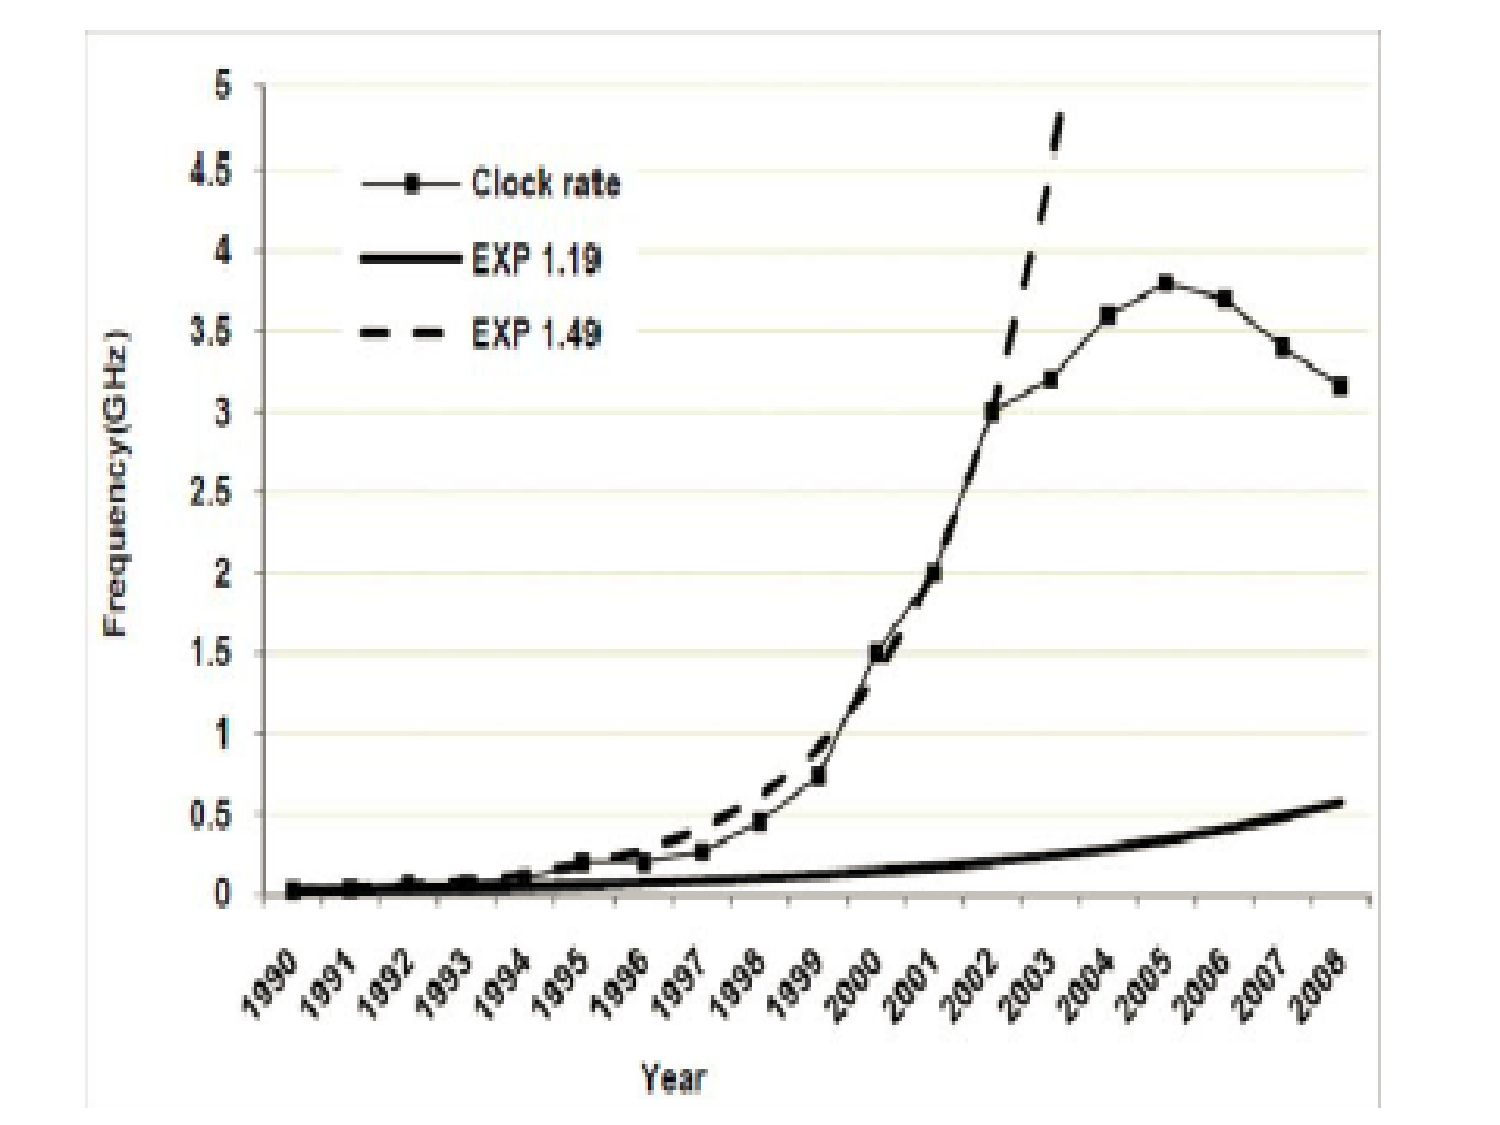
\includegraphics[width=40ex]{Ch1Figs/FreqGraph}
\column{0.57\textwidth}
        \begin{itemize}
            \item \emph{Technology} (process shrinkage): every generation 
                    transistors' \emph{switching speed increases $41\%$}.\medskip

%                    \item Impact blunted in the future due to \emp{wire delays}
%                                (do not scale)
%                            because speed of wire transmission grows much slower than
%                            switching speed.
%                \end  {itemize}\medskip
            \item \emph{Pipeline Depth:} more stages $\Rightarrow$
                            less complex $\Rightarrow$ less gates/stage
                \begin{itemize}
                    \item \# of gates delays dropped by $25\%$ every process generation.
                \end  {itemize}\medskip

                \item \emph{Improved Circuit Design} 
        \end  {itemize}\bigskip
\end{columns}
\pause

Clock Rate Increase is Not Sustainable:
\begin{itemize}
    \item \emp{Deeper pipelines}: difficult to build useful stages with $<$ 10 gates
    \item \emp{Wire delays:} wire-transm speed $\uparrow$ much 
            slower than switching,
    \item Circuits clocked at \emp{higher rates consume more power}!  
\end  {itemize}

\end{frame}

\begin{frame}[fragile,t]
\frametitle{Processor: Feature Size \& Number of Transistors}

\begin{columns}
\column{0.65\textwidth}
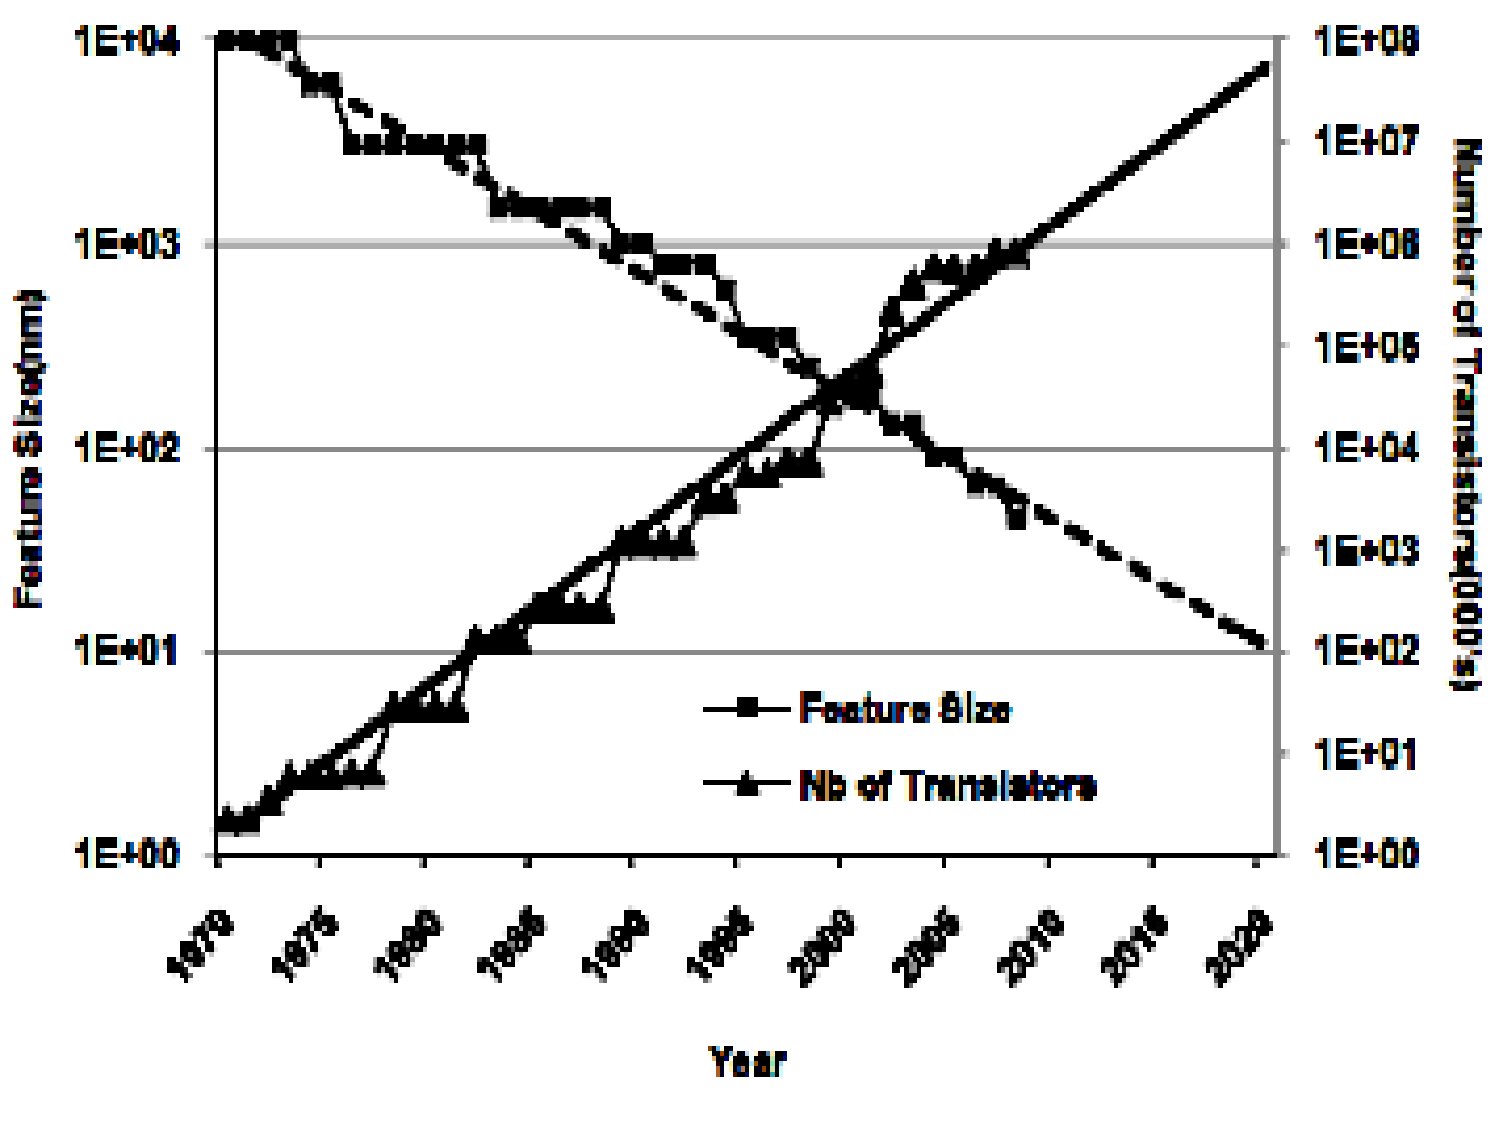
\includegraphics[width=47ex]{Ch1Figs/FeatureSize}
\column{0.4\textwidth}
%\begin{scriptsize}
        \begin{itemize}
            \item new process generation every 2 years\smallskip
                
            \item feature size reduced $30\%$ every generation

            \item \# of transistors doubles every 2 years (Moore's low).\\
                    1 Billion in 2008. 
        \end  {itemize}
%\end{scriptsize}
\end{columns}
\vspace{-2ex}

Each process generation offers new resources.
\emp{How best to use the $>100$ billion transistors? Large-Scale CMPs (100s-1000s cores)}:
\begin{itemize}
    \item more cache, better memory-system design
    \item fetch and decode multiple instr per clock
    \item running multiple threads per core and on multiple cores
\end  {itemize} 

\end{frame}

\subsection{Memory}

\begin{frame}[fragile,t]
\frametitle{Memory Systems}

\begin{itemize}
    \item \emp{(Main) Memory Wall:} growing gap between processor and memory speed.
            Processor cannot execute faster than memory system can deliver data 
            and instructions!\bigskip

    \item Want Big, Fast \& Chip Memory System\smallskip
    \begin{itemize}
        \item access time 
                increases with memory size as it is dominated by 
                wire delays$\Rightarrow$ this will not change in future technologies\smallskip
%(address decoding, address line propagation, bit-line propagation) 
        \item multi-level hierarchies (relies on principle of locality)\smallskip
        \item efficient management is KEY, e.g., cache coherence.\smallskip
        \item Cost and Size memories in a basic PC in 2008:
    \end  {itemize} 
\end{itemize}
\bigskip

\begin{tabular}{|l|l|l|l|l|}\hline
Memory & Size  & Marginal Cost & Cost Per MB & Access Time \\\hline
L2 Cache & 1MB & \$20/MB & \$20 & 5nsec \\\hline
Main Memory & 1 GB & \$50/GB & 5c & 200 nsec \\\hline
Disk & 500GB & \$100/500GB & 0.02c & 5 msec \\\hline
\end{tabular}

\end{frame}


\begin{frame}[fragile,t]
\frametitle{Memory Wall? Which Memory Wall??}

\begin{itemize}
            \item \emph{DRAM density increases $4\times$ every 3 years, BUT} \smallskip

            \item \emp{DRAM speed $\uparrow$ only with $7\%$ per year!} 
                    (processor speed by $50\%$) 

            \item \alert{Perception was that Memory Wall will last forever!}

            \item \emph{Memory Wall Stopped Growing around 2002}.
    
            \item Multi/Many-Cores $\Rightarrow$ shifted from Latency 
                    to \emp{Bandwidth WALL}
\end  {itemize}
\vspace{-3ex}

\begin{columns}
\column{0.65\textwidth}
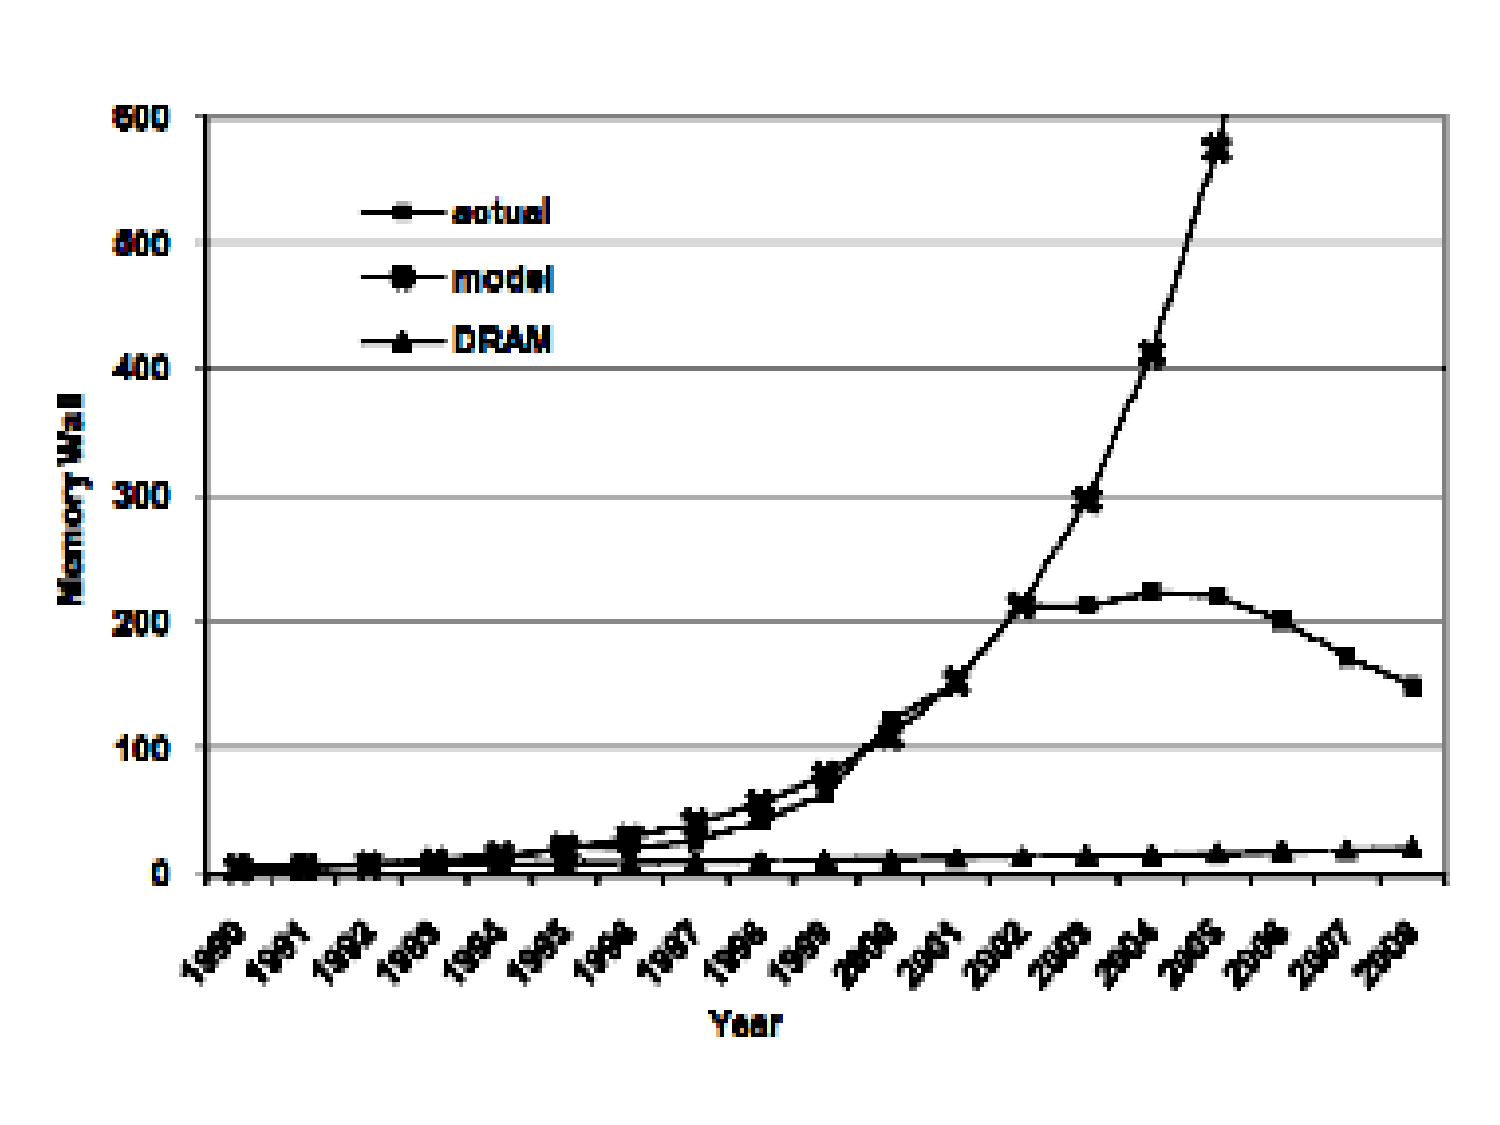
\includegraphics[width=50ex]{Ch1Figs/MemWall}
\column{0.3\textwidth}
\begin{scriptsize}
\begin{itemize}
\item {\tt MemoryWall = mem\_cycle/ proc\_cycle} \smallskip
\item[1990] {\tt MemoryWall = 4} (25MHz,150ns)
\item[2002] exponential growth {\tt MemoryWall = 200} 
\item Stalled since then.
\item If trend continues: 1 Terabit Main Memory by 2021.
\end{itemize}
\end{scriptsize}
\end{columns}

\end{frame}


\begin{frame}[fragile,t]
\frametitle{Disk Memory}

\begin{itemize}
            \item \emph{Historically disk performance improved by $40\%$ per year} \smallskip

            \item {\tt DiskTime=AccessTime+TransferTime} ({\scriptsize {\tt AccessTime=Seek+Latency}})

            \item Historically, transfer time have dominated, but

            \item Today: transfer and access time are of the same \alert{msecs} order
    
            \item Future, Access Time will dominate, but proc-disk gap still large
\end  {itemize}

\begin{columns}
\column{0.5\textwidth}
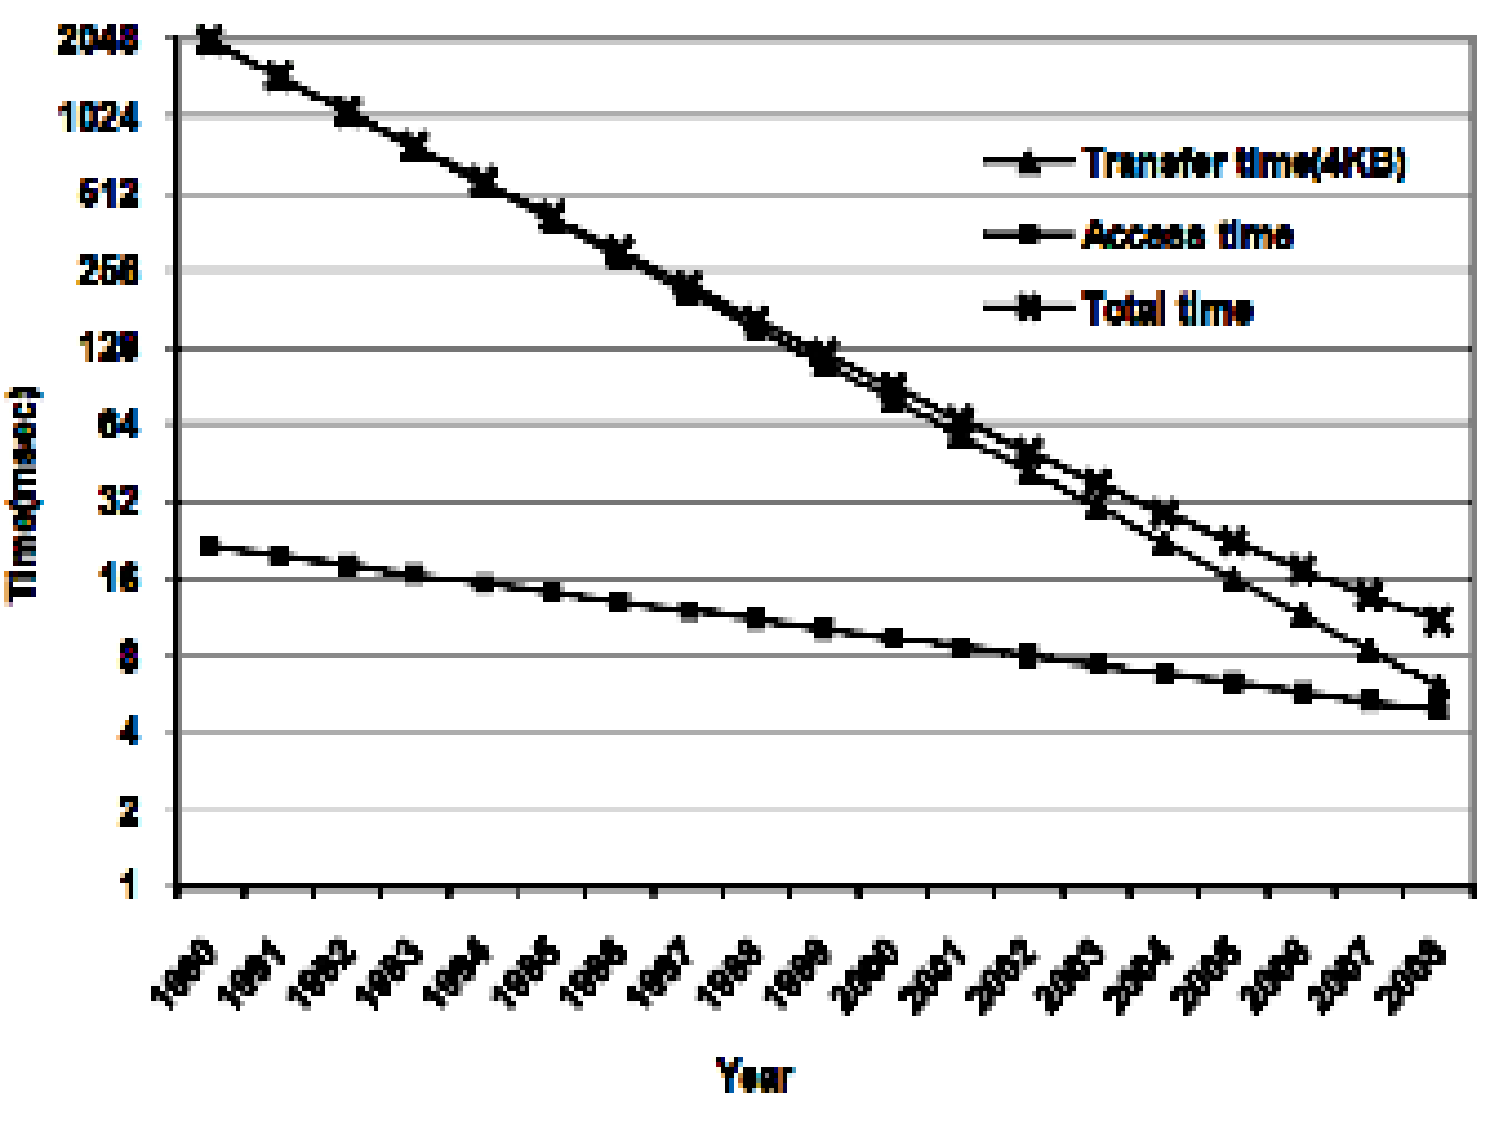
\includegraphics[width=33ex]{Ch1Figs/DISK}
\column{0.5\textwidth}
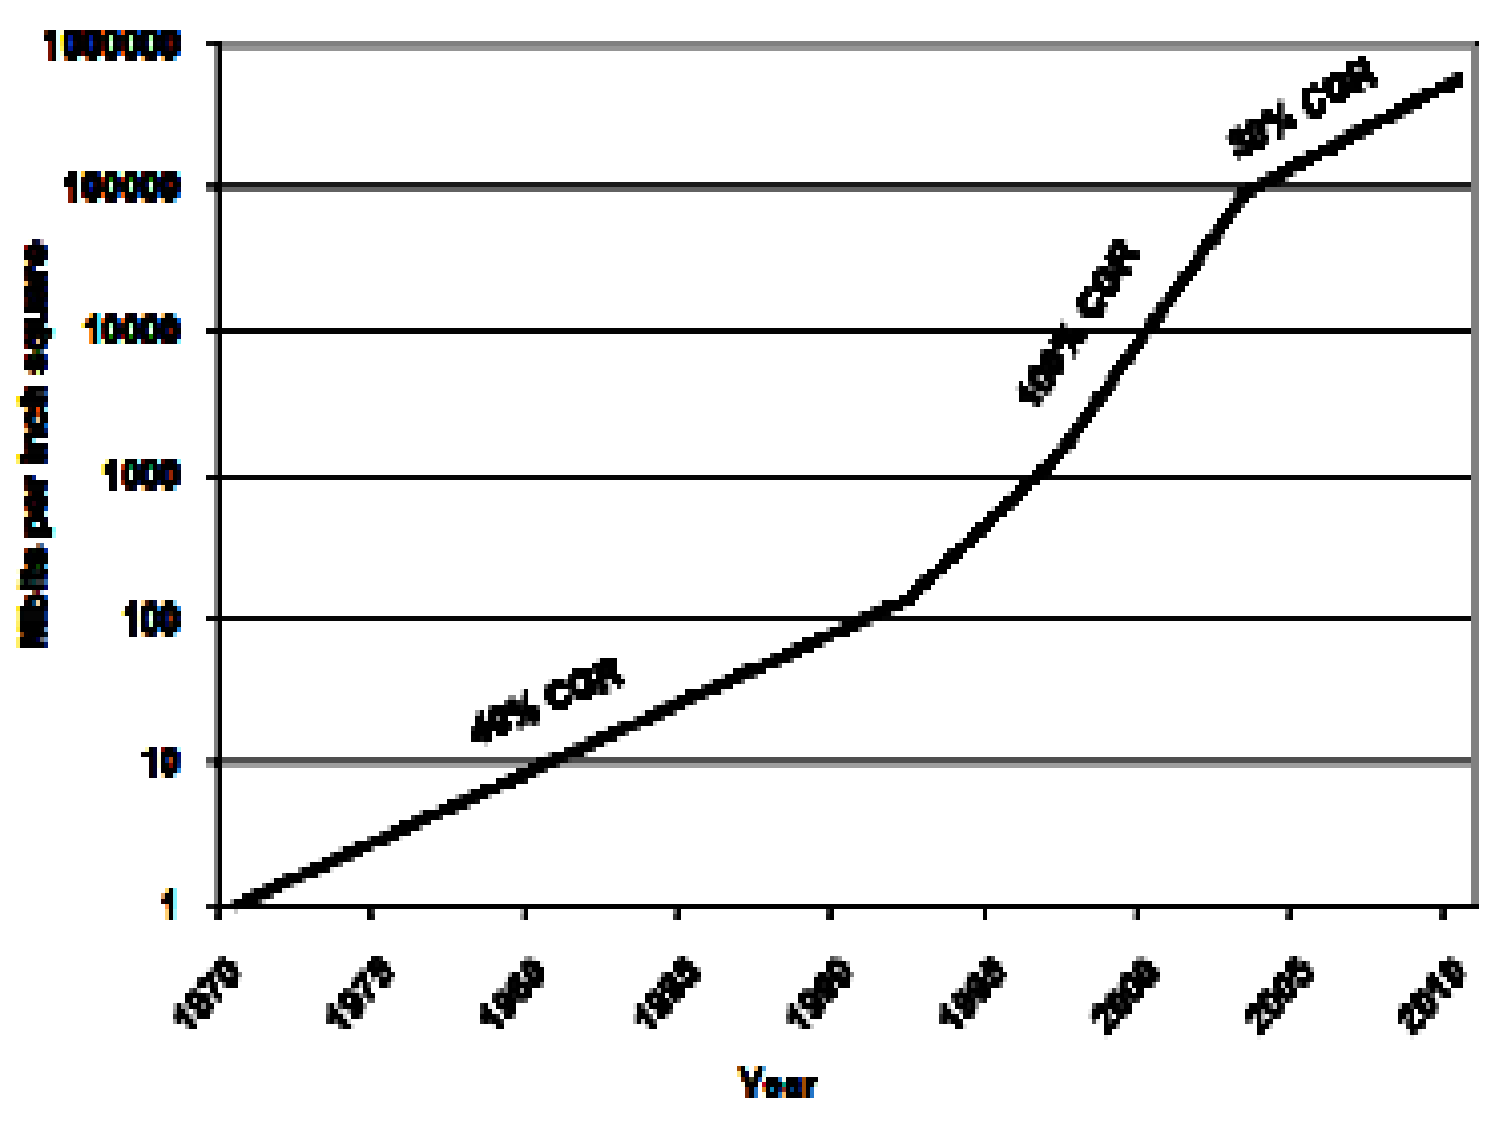
\includegraphics[width=33ex]{Ch1Figs/Disk2}
\end{columns}

{\scriptsize Seek Time: head to reach right track, latency: time to reach the first record on track, both depend on rotation speed \& independent on block size}.

\end{frame}

\subsection{Interconnect}
\begin{frame}[fragile,t]
\frametitle{Interconnection Networks}

Present at many layers:
\begin{itemize}
            \item \emp{On-Chip Interconnects:} forward values between pipeline stages, AND between execution units AND connect cores to shared cache banks. \smallskip

            \item \emp{System Interconnects:} connect processors (CMPs) to memory and IO

            \item \emp{I/O Interconnects}, usually bus e.g., PCI, connect various 
                    devices to the System Bus
            \item \emp{Inter-Systems Interconnects:} connect separate systems (chassis or boxes) \& include
                \begin{itemize}
                    \item \emph{SANs:} connect systems at very short distance
                    \item LANs, WANs (not interesting for us).
                \end  {itemize}

            \item Internet: global world-wide interconnect (not interesting for us).
\end  {itemize}

\end{frame}

%%%%%%%%%%%%%%%%%%%%%%%%%%%%%%%%%%%%%%%%%%%%
%%%%%%%%%%%%%%%%%%%%%%%%%%%%%%%%%%%%%%%%%%%%

\section{Technological Challenges/Constraints}

\begin{frame}[fragile]
	\tableofcontents[currentsection]
\end{frame}


\begin{frame}[fragile,t]
\frametitle{Technological Contraints}

\begin{itemize}
    \item In the Past: tradeoff between cost (area) and time (performance).\bigskip

    \item Today: design is challenged by several technological limits\smallskip
        \begin{itemize} 
            \item \alert{Major new contraint is Power}\smallskip
            \item wire delays\smallskip
            \item reliability\smallskip
            \item complexity of design
        \end  {itemize}\bigskip

    \item Architecture can play a significant role to maintain viability
            of CMOS technology for years to come
\end{itemize}
\end{frame}

\subsection{Power}

\begin{frame}[fragile,t]
\frametitle{Power}

\begin{itemize}
    \item \emp{\tt Total Power = Dynamic + Static (Leakage)}\\
                        $P_{dynamic} = \alpha C V^2 f$ 
                        consumed by a gate when it switches state\\
                        $P_{static}  = V I_{sub} \sim V e^{-k V_T / T}$ 
                        (caches)\medskip

    \item Dynamic power 
            favors parallel processing over higher clock rate
            \begin{itemize}
                \item $P_{dynamic} \sim F^3$ mostly dissipated in processor\pause
                \item replicate a uniprocessor 4 time $\Rightarrow$ 
                        $4\times$ speedup @ $4\times$ power
                \item increase clock 4 times $\Rightarrow$ 
                        $4\times$ speedup @ $64\times$ dynamic power!
            \end  {itemize}\medskip

    \item Static Power: dissipated in all circuits,  
                at all time, nomatter of frequency and whether
                it switches or not.
            \begin{itemize}
                \item negligible 15 years ago, but as feature size 
                        decreased so did the threshold voltage $V_T$ 
                        every generation
                \item \alert{Recently overtook dynamic power as major 
                        source of dissipation!}
            \end{itemize}\medskip

    \item \emp{Power/Energy are Critical Problems}\\ 
                e.g., costly \& many battery operated devices.
%            \begin{itemize}
%                \item Power must be dissipated otherwise temperature
%                        goes up \& affects performance, correctness and
%                        may possibly destroy the circuit, short or long term. 
%                \item Energy depends on power and speed. Costly \& 
%                        many devices are battery-operated devices.
%
%            \end  {itemize}
\end  {itemize}


\end{frame}


\subsection{Reliability}

\begin{frame}[fragile,t]
\frametitle{Reliability}

\begin{itemize}
    \item \emp{Transient Failures (Soft Errors):}
        \begin{itemize}
            \item Charge stored in a transistor \emp{\tt Q = C V}
            \item Supply voltage $V$ decreases every generation\\
                    (consequence of features-size shrinking)
            \item As Q decreases, it is easier to flip bits
            \item Corruption Sources: cosmic rays, alpha particles
                    radiating from the packaging material, electrical noise
            \item Device operational but values have been corrupted
            \item DRAM/SRAM error detection and correction capability
        \end  {itemize}\medskip

    \item \emp{Intermittent/Temporary Failures:}
            \begin{itemize}
                \item last longer, should try to continue execution
                \item aging or temporary environmental variation, e.g., temperature
            \end  {itemize}\medskip

    \item \emp{Permanent Failures:} device will never function again,
                must be isolated \& replaced by spare\medskip

    \item \emph{Chip Mutiprocessors: promote better reliability}
            \begin{itemize}
                \item using threads for redundant execution, 
                \item faulty cores can be disabled $\Rightarrow$ 
                        natural failsafe degradation
            \end  {itemize}
\end  {itemize}
\end{frame}

\subsection{Wire Delays}
\begin{frame}[fragile,t]
\frametitle{Wire Delays}

\begin{itemize}
    \item Miniaturization $\Rightarrow$ transistors switch faster,
            but the propagation delay of signals on wire does not 
            scale as well.\medskip

    \item Wire Delay Propagation $\sim R C$. $R \sim L / CS_{area}$.
            Miniaturization $\Rightarrow$ cross-section area keeps shrinking
                each generation, annuls the benefit of length shrinking. \medskip

    \item Wires can be pipelined like logic.\medskip

    \item Deeper pipelines are better because communication
            limited to only few stages.\medskip

    \item \emph{Impact of wire delays also favors multiprocessors,
            since communication traffic is hierarchical:}
            \begin{itemize}
                \item most communication is local 
                \item inter-core communication is occasional
            \end  {itemize}

\end  {itemize}
\end{frame}

\subsection{Design Complexity}
\begin{frame}[fragile,t]
\frametitle{Design Complexity}

\begin{itemize}
    \item Design Verification has become the dominant cost of chip
            development today, major design constraint.\medskip

    \item \emp{Chip density increases much faster than the productivity 
                of verification engineers} (new tools and speed of systems):
            \begin{itemize}
            \item register-transfer language level, i.e., logic is correct 
            \item core level, i.e., correctness of forwarding, memory disambiguation,
            \item multi-core level, e.g., cache coherence, memory consistency.
            \end  {itemize}\medskip

    \item Vast majority of chip resources dedicated to storage
            also due to verification complexity:
            \begin{itemize}
            \item trivial to increase the size of: 
                caches, store buffers, load/store/ fetch queues, reorder buffers,
                    directory for cache coherence, etc.
            \end  {itemize}\medskip

    \item \emph{Design Trend Favors Multiprocessors:}
            easier to replicate the same structure multiple times
            than to design a large, complex one.
\end  {itemize}
\end{frame}

\subsection{CMOS Endpoint}
\begin{frame}[fragile,t]
\frametitle{CMOS (Endpoint) Meets Quantum Physics}

\begin{itemize}
    \item CMOS is rapidly reaching the limits of miniaturization,\medskip

    \item Feature size: half pitch distance (half the distance between
            two metal wires). Gate length $\sim 1/2$ feature size.\medskip

    \item If present trends continues feature size $< 10 nm$ by 2020\medskip

    \item Radius of atom: $0.1 \sim 0.2 nm$ $\Rightarrow$ gate length quickly
            reaches atomic distances that are governed by quantum physics,
            i.e., binary logics replaced with probabilistic states.\medskip

    \item Not clear what will follow (?)
\end  {itemize}
\end{frame}

%%%%%%%%%%%%%%%%%%%%%%%%%%%%%%%%%%%%%%%%%%%
%%%%%%%%%%%%%%%%%%%%%%%%%%%%%%%%%%%%%%%%%%%
%%%%%%%%%%%%%%%%%%%%%%%%%%%%%%%%%%%%%%%%%%%
\section{Performance}

\begin{frame}[fragile]
	\tableofcontents[currentsection]
\end{frame}

\subsection{Metrics}

\begin{frame}[fragile,t]
\frametitle{Performance Metrics \& Benchmarking}

Performance Metrics:
\begin{itemize}
    \item[1] \emp{Execution Time or Latency or Response Time}: 
            time to complete a task $T_{exec}$.
            Is the ultimate measure of performance\medskip

    \item[2] \emp{Throughput}: number of tasks per day, hour, sec
        \begin{itemize}
            \item not the same as, e.g, dual-core vs doubled-frequency uniprocessor.
        \end  {itemize}\medskip
\end{itemize}

Benchmarking:\smallskip
\begin{itemize}
    \item Source Code:\pause because some machines are designed with
            a compiler in mind and are easier to optimize code for.\smallskip

    \item Benchmark Suites:\pause many \& large programs to avoid fine tuning
        \begin{itemize}
            \item[SPEC] Standard Performance Evaluation Corporation:
                \begin{itemize}
                    \item scientific/engineering/general purpose
                    \item integer and floating point
                    \item new datasets and applications so 
                            many years,e.g, 98/2000/2006
                \end  {itemize}
            \item[TPC] Transactional Processing Council:
            \item Embedded Benchmarks
            \item Media Benchmarks
        \end  {itemize}
\end  {itemize}
\end{frame}


\begin{frame}[fragile,t]
\frametitle{Reporting Performance of a Set of Programs}

Let $T_i$ be the execution time of program $i$:
\begin{itemize}
    \item[1] Weighted Arithmetic or Harmonic Mean:\\
            $\sum_i T_i/N$ or $\sum_i T_i \times W_i$ or $N / (\sum_i )$\\
            \alert{Program with longest execution dominates the rest}\medskip

    \item[2] Speedup against a reference machine $R$:\\
                $S_i = T_{R,i} / T_i$\medskip

    \item[3] Arithmetic and harmonic ($N/(\sum_i 1/S_i)$) means of speedups: 
                \alert{Problem: the comparison
                of two different machines yields a different conclusion
                with a different reference machine.}\medskip
    \item[4] \emph{Geometric Mean, i.e., $S_g = \sqrt[N]{\prod_{i=1}^N S_i}$:}
                \begin{itemize}
                    \item does not have the above problem, and
                    \item are composable, i.e., $S_{g_{I\cup II}} = S_{g_I} S_{g_{II}}$
                \end  {itemize}
\end{itemize}

\end{frame}

\begin{frame}[fragile,t]
\frametitle{Fundamental Performance Equations for CPU}

\centering{$T_{exe} = IC \times CPI \times T_c$}
\begin{itemize}
    \item[IC] instruction count: depends on compiler and ISA
    \item[CPI] clock per instruction: depends on 
                instruction mix, ISA, and implementation
    \item[Tc] cycle time: depends on implementation complexity and technology.
\end{itemize}\bigskip

\emp{CPI impossible to estimate directly with complex OoO and cache hierarchies.}
\emph{Often used instead of execution time}, i.e., $CPI = T_{exe} / (IC \times T_c)$
\bigskip


When processor executes more than one instructions per clock
use IPC (instructions per clock): $T_{exe} = (IC \times T_c) / IPC$

\end{frame}

\subsection{Amdhal and Gustafson's Laws}

\begin{frame}[fragile,t]
\frametitle{Amdahl's Law}
\vspace{-5ex}
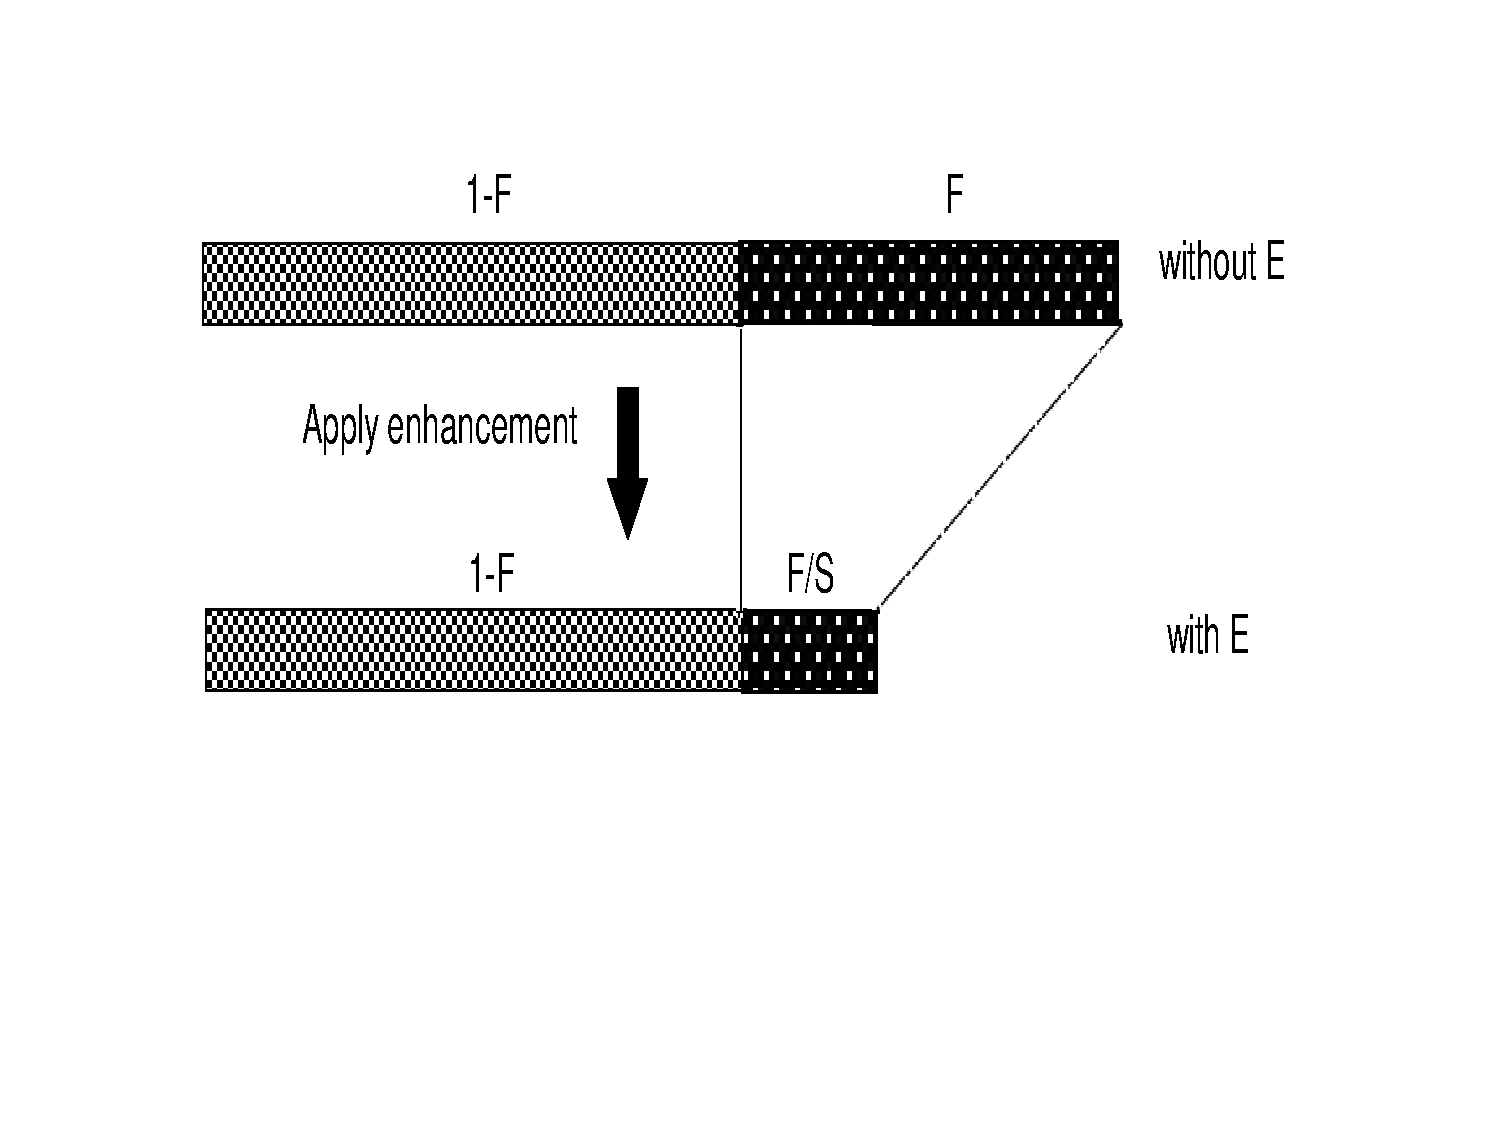
\includegraphics[width=47ex]{Ch1Figs/Amdhal}
\vspace{-7ex}

Enhancement accelerates a fraction $F$ of the task by a factor $S$:\bigskip

\centering{$T_{exe}(with E) = T_{exe}(without E)\times[(1-F) + \frac{F}{S}]$}\bigskip

\centering{$Speedup(E) = \frac{T_{exe}(without E)}{T_{exe}(with E)} = \frac{1}{(1-F)+\frac{F}{S}}$}

\end{frame}

\begin{frame}[fragile,t]
\frametitle{Amdahl's Law}

\begin{itemize}
    \item[1] Improvement is limited by the $1-F$ part of the execution 
                that cannot be optimized:
                $Speedup(E) < \frac{1}{1-F}$\medskip

    \item[2] Optimize the common case \& execute the rare case in software.

    \item[3] Low of diminishing returns\smallskip

\end{itemize}

\vspace{-4ex}
\begin{columns}
\column{0.7\textwidth}
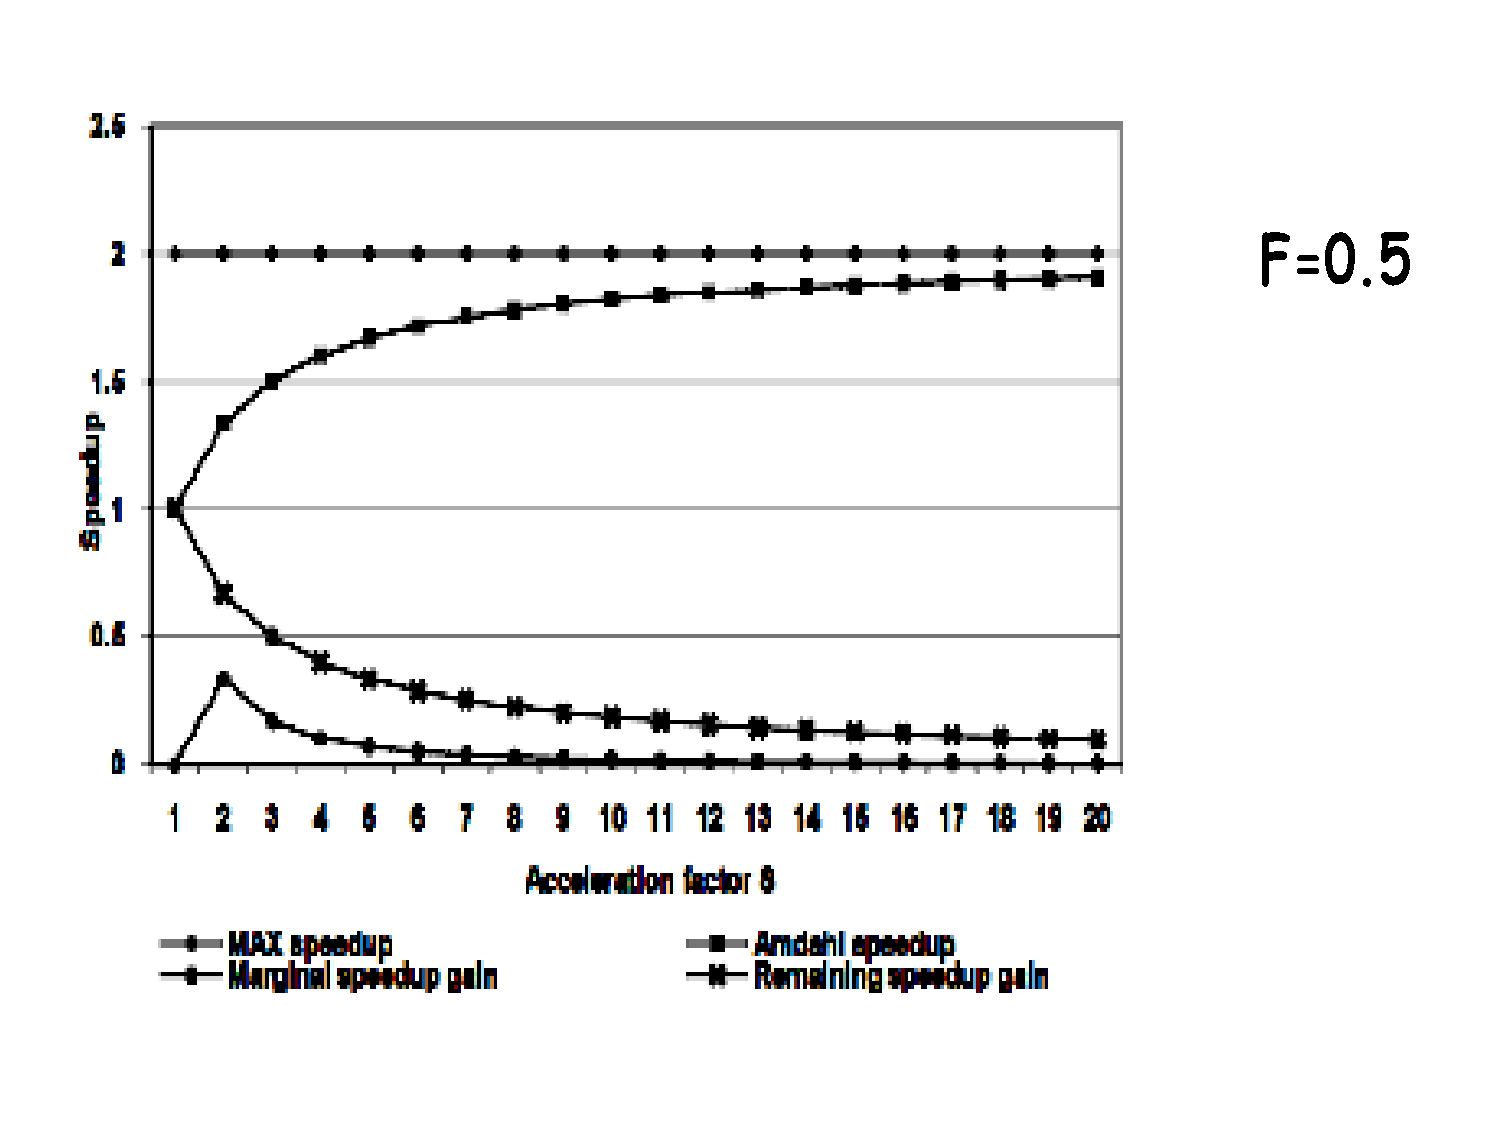
\includegraphics[width=55ex]{Ch1Figs/AmdhalDimRet}\pause
\column{0.5\textwidth}\vspace{-3ex}
\begin{itemize}
    \item every increment of $S$ consumes new resources \& becomes less rewarding: 
    \item $S = 2 \Rightarrow 33\%$ speedup,
    \item $S = 5 \Rightarrow 6.67\%$ speedup.
\end{itemize}
\end{columns}

\end{frame}


\begin{frame}[fragile,t]
\frametitle{Amdahl's Law: Parallel Speedup}

\centering{$S_P = \frac{T_1}{T_P} = \frac{P}{F+P(1-F)} < \frac{1}{1-F}$}\medskip

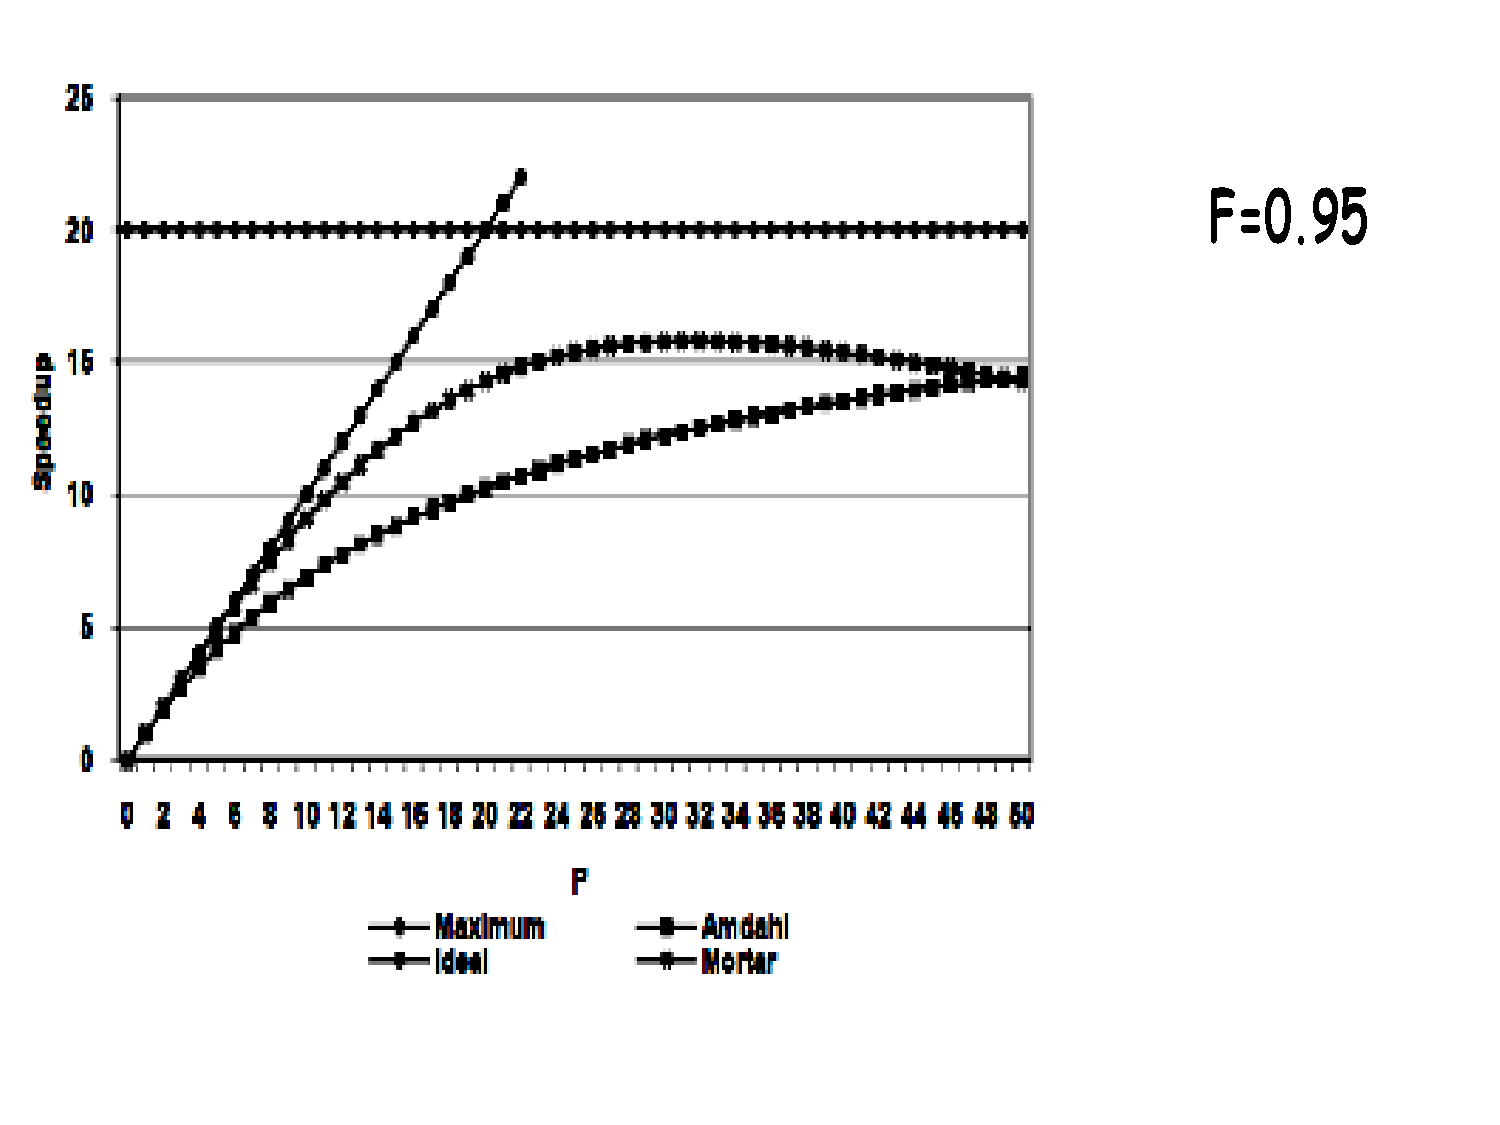
\includegraphics[width=44ex]{Ch1Figs/ParSpeedup}
\vspace{-5ex}

Typically: speedup is sublinear, e.g., due to inter-thread communic.\medskip 

Sometimes speedup can be superlinear due to cache effects.\medskip
 
\alert{Unforgiving Law: even if $99\%$ can be parallelized, speedup cannot be $> 100$. Overall not very hopeful!}

\end{frame}

\begin{frame}[fragile,t]
\frametitle{Gustafson's Law}

Redefines Speedup. Rationale:
\begin{itemize}
    \item workloads go up with the number of cores
    \item execution time on parallel machine with P processors: $T_p = s + p$
    \item where $s$ and $p$ are the times of the serial and parallel code.
    \item Hence execution time on one processor is $T_1 = s + pP$.
    \item Now let $F = p/(s+p)$ $\Rightarrow$ 
            \emp{$S_p = \frac{s+pP}{s+p} = 1 + F(P-1)$}
\end  {itemize}
\vspace{2ex}

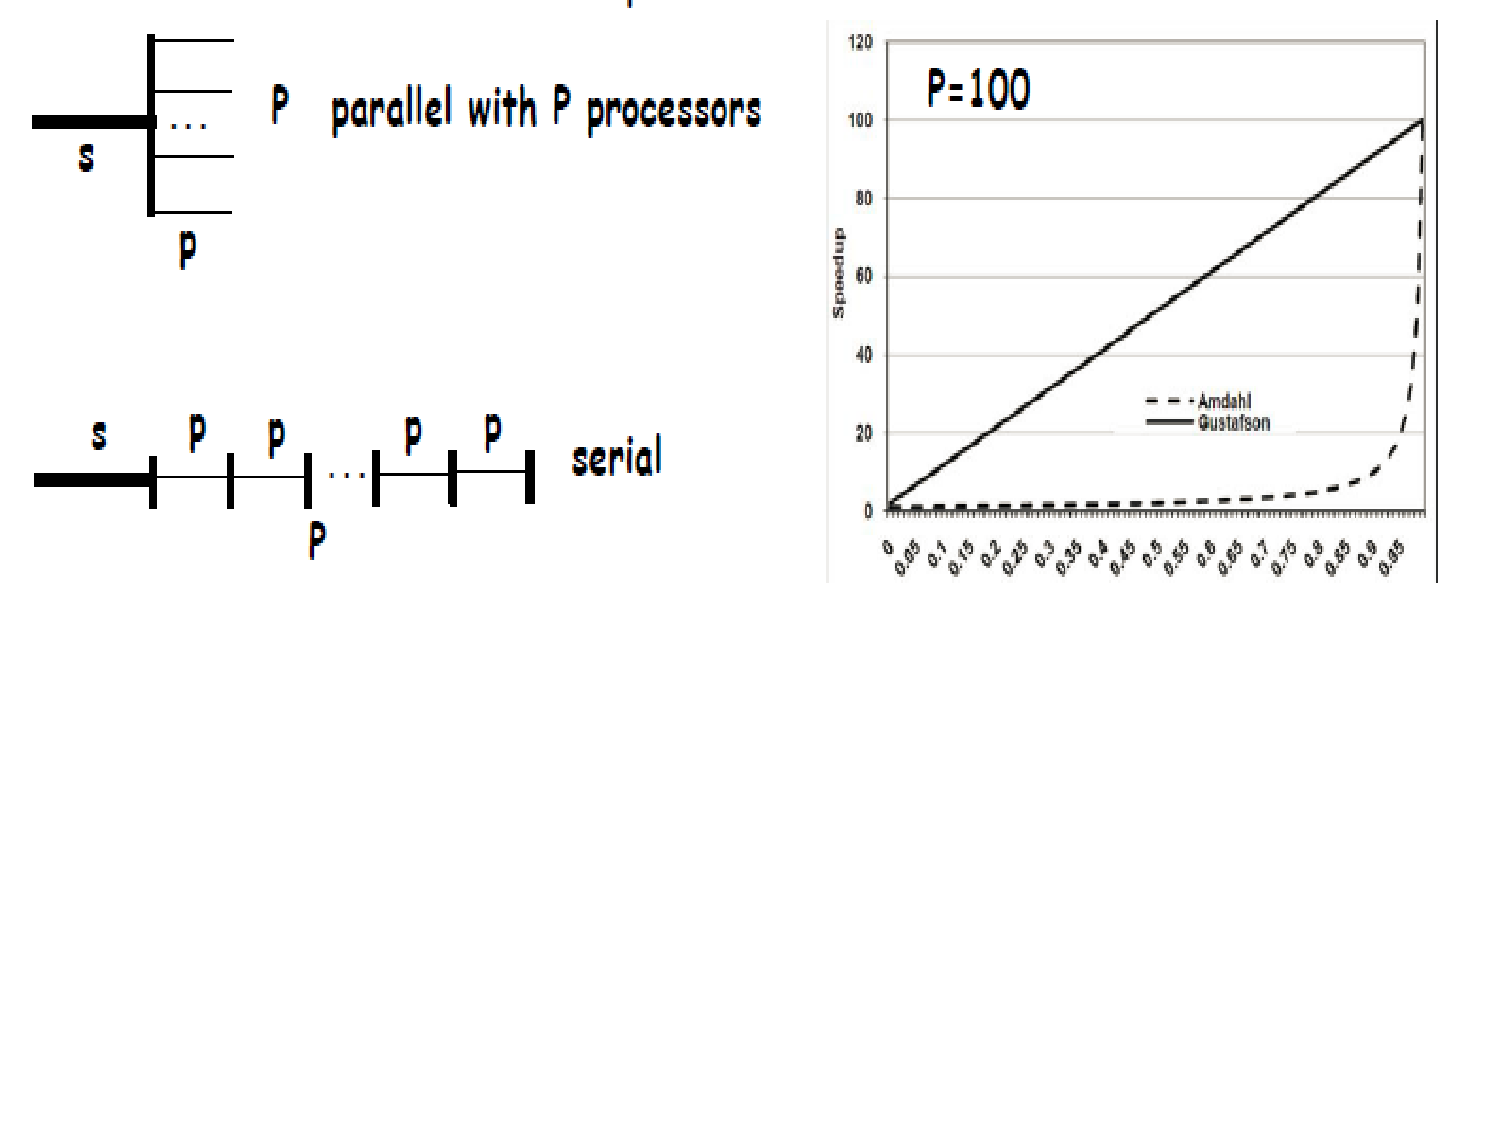
\includegraphics[width=59ex]{Ch1Figs/AmdhalGustaff}


\end{frame}


%%%%%%%%%%%%%%%%%%%%%%%%%%%%%%%%%%%%%%%%%%%
%%%%%%%%%%%%%%%%%%%%%%%%%%%%%%%%%%%%%%%%%%%
%%%%%%%%%%%%%%%%%%%%%%%%%%%%%%%%%%%%%%%%%%%

\section{Parallelism In Architectures: Vector \& Array Processors}

\begin{frame}[fragile]
	\tableofcontents[currentsection]
\end{frame}


\begin{frame}[fragile,t]
\frametitle{Scalar Multiprocessors}

\begin{itemize}
            \item Most Successful Architectures: Scalar Processor
                \begin{itemize}
                    \item instruction operates on scalar operands, 
                            e.g., {\tt ADD R1, R2, R3 $\Rightarrow$ R1 := R2 + R3}
                    \item execute multiple scalar instructions at a time:
                    \begin{itemize}
                        \item pipelining, 
                        \item superscalar
                        \item superpipelining
                        \item take advantage of instruction-level (intra-thread) 
                                parallelism (ILP).
                    \end  {itemize}
                \end  {itemize}

            \item Chip Multiprocessors (CMPs) exploits inter-thread parallelism:
                    \begin{itemize}
                        \item i.e., different threads running in parallel. 
                        \item multiple scalar processors running in parallel
                    \end  {itemize}
\end  {itemize}

\end{frame}

\begin{frame}[fragile,t]
\frametitle{Vector and Array Processors}

\begin{itemize}
    \item Able to execute instructions on entire vectors rather than scalars\medskip
    \begin{itemize}
        \item {\tt ADDV V1,V2,V3} has semantics: 
                {\tt V1[i] := V2[i] + V3[i] $\forall i$}\smallskip
        \item {\tt V1}, {\tt V2}, and  {\tt V3} denote vectors of same 
                length and scalar type, that can be specified either 
                as vector registers or\smallskip
        \item by a \emp{\bf base address}, a vector \emp{\bf length} 
                and a \emp{\bf stride} operand,\smallskip
        \item where length and address can be held in special control registers.
    \end{itemize}\medskip

    \item Very old architecture, 1960s, CDC Star, Cray, IBM 3033.\\
            Required a vectorizing compiler to extract vector parallelism.\medskip 
%predate superscalar processors.\medskip

    \item \alert{Reappearing in commodity markets --
                    multimedia applic (DSP).} 
\end  {itemize}

% Vector instructions executed by pipelines or parallel arrays
%\begin{columns}
%\column{0.9\textwidth}
%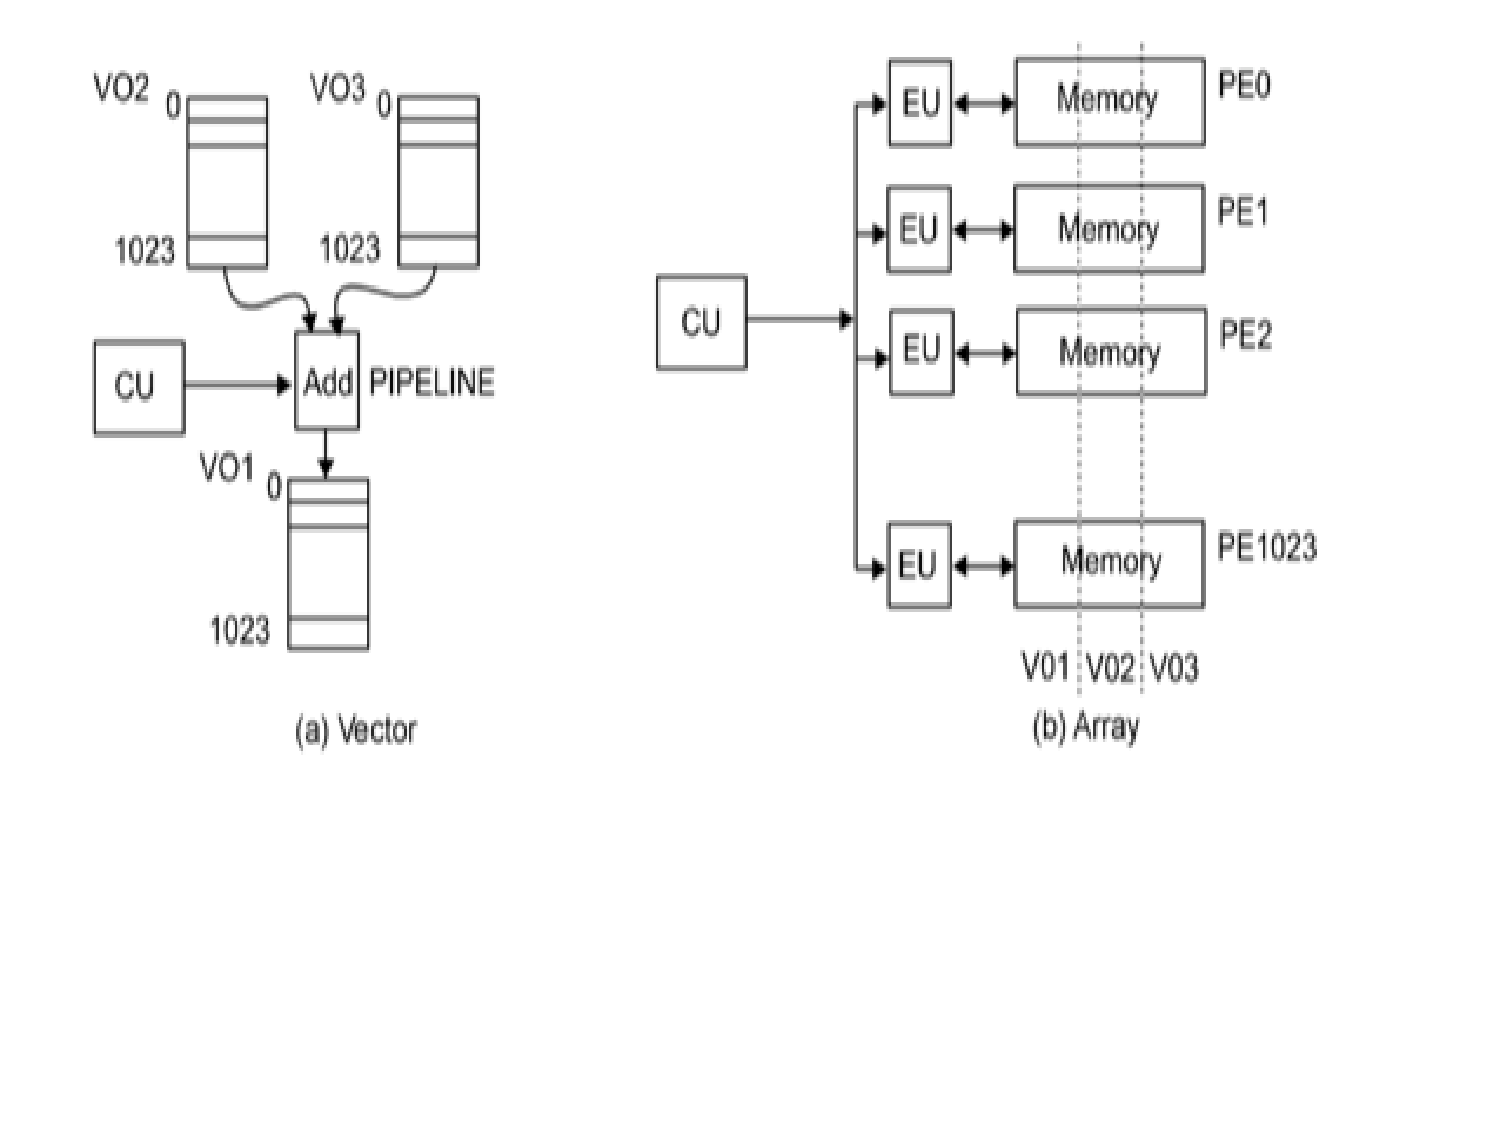
\includegraphics[width=65ex]{Ch1Figs/VectorMachine}
%\column{0.1\textwidth}
%\end{columns}
\vspace{-1ex}

\begin{columns}
\column{0.5\textwidth}
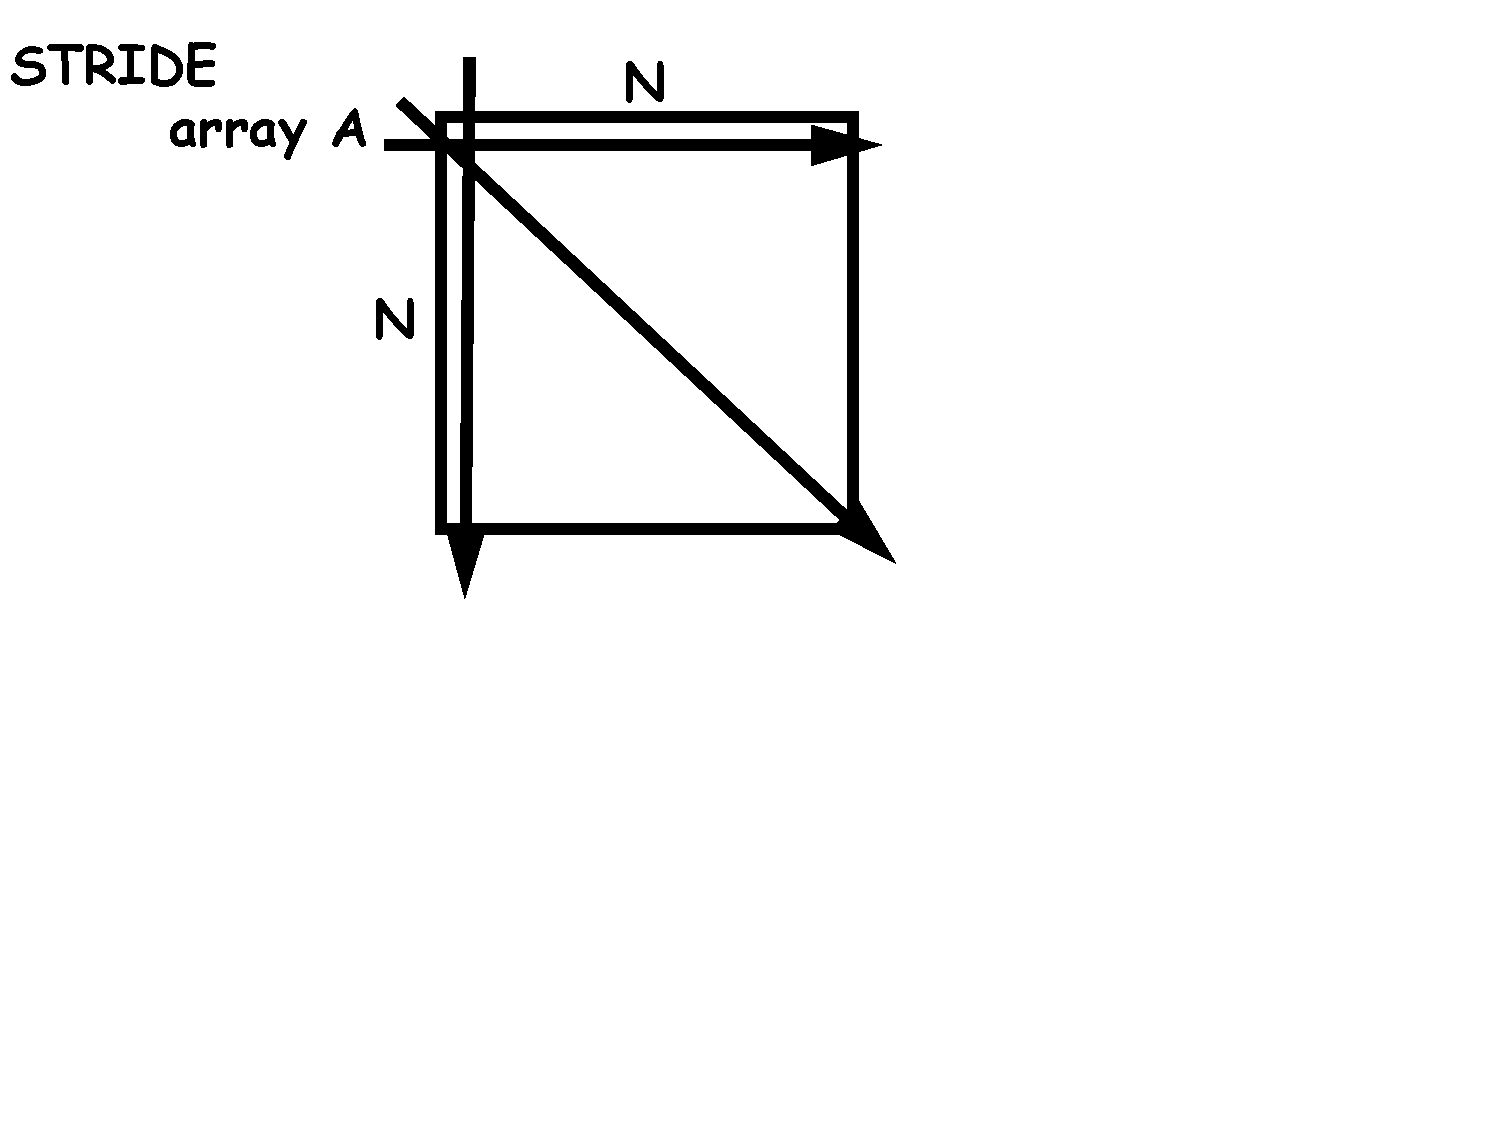
\includegraphics[width=55ex]{Ch1Figs/MatrixStrides}\pause
\column{0.5\textwidth}
\vspace{-15ex}

{\tt N$\times$N} matrix\\
row: stride {\tt 1}\\
column: stride {\tt N}\\
diagonal: stride {\tt N-1} or {\tt N+1} 
\end{columns}


\end{frame}


\begin{frame}[fragile,t]
\frametitle{Vector and Array Processors}

\begin{columns}
\column{0.35\textwidth}
\vspace{-13ex}

If ADD has 10 stages.\\
Total Execution Time:\\
$T_{exe} = 10 + 63 = 9 + 64$\\\medskip

In general: $T_{exe} = T_{start}+N$,\\
where $N$ is vector's length.
\column{0.7\textwidth}
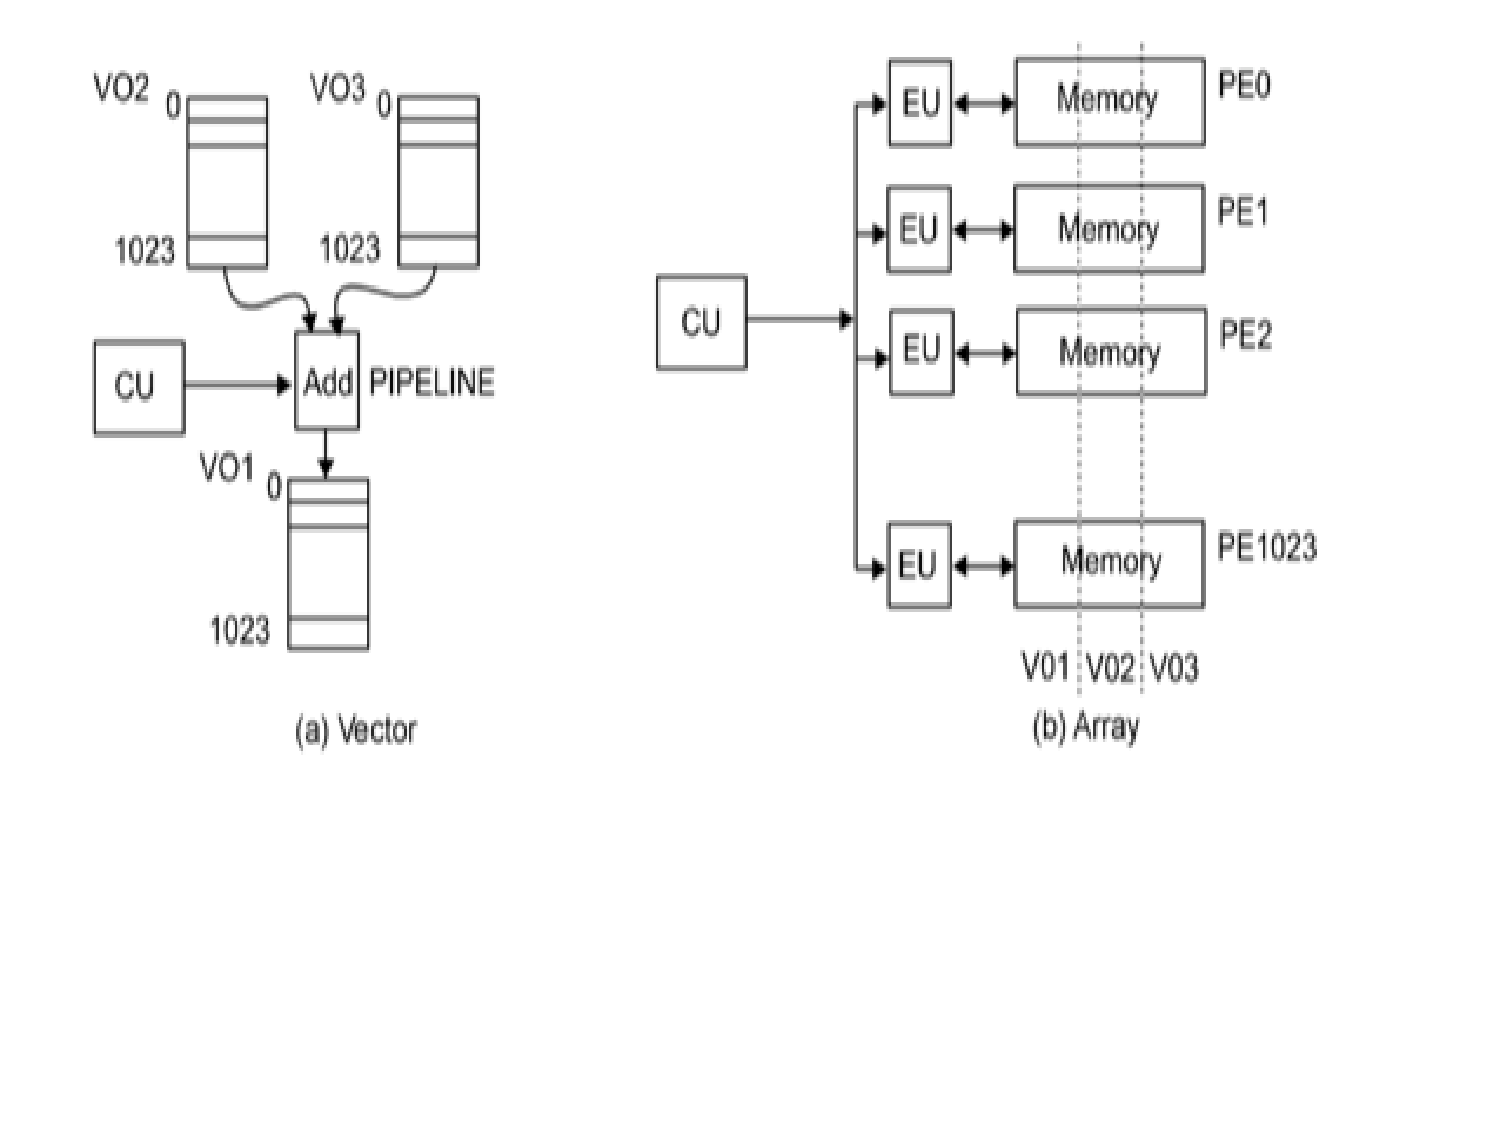
\includegraphics[width=53ex]{Ch1Figs/VectorMachine}
\end{columns}
\vspace{-10ex}
After vector's startup time, i.e., the time to get the first result,
scalar results are computed one per clock:\\

\centering{\emp{\tt T$_{vector}$ = Vector Length + Startup Time}}

\end{frame}


\begin{frame}[fragile,t]
\frametitle{Load/Store Vector Architecture}

\begin{itemize}
    \item vector registers + scalar registers
    \begin{itemize}
        \item each vector register can hold consec vector components
                fetched from memory, 
                e.g, 8 vector registers of 64 components each
        \item 1 READ and 1 WRITE port per vector register, 
                connected to function units via crossbar interconnect
                (all registers to all units).
    \end  {itemize}\medskip

    \item Vector functional units are specialized and deeply pipelined, and
            act on operands in vector registers
\end  {itemize}

\begin{block}{HL Code{\tt~~~~~~~~}Machine Code{\tt~~~~~~~~~}Comments}
\begin{columns}
\column{0.24\textwidth}
\begin{colorcode}[fontsize=\scriptsize]
for(i=0; i<2048; i++)
  Y[i] = a*X[i] + Y[i]
\end{colorcode} 
\column{0.24\textwidth}
\begin{colorcode}[fontsize=\scriptsize]
    ADDI  R6,R0,#1
LOOP:
    L.V   V1,0(R1),R6
    MUL.V V2,V1,F0
    L.V   V3,0(R2),R6
    ADD.V V4,V2,V3
    S.V   V4,V2,R6
    SUBBI R1,R1,\#512
    SUBBI R2,R2,\#512
    SUBBI R3,R3,2
    BNEZ  R3,LOOP
\end{colorcode} 
\column{0.47\textwidth}
\begin{colorcode}[fontsize=\scriptsize]
//sets R6 to 1 (the stride)
//load slice of vector X of  
//  base 0(R1) \& stride R6  
//multiply X with scalar in F0 
//load slice of vector Y
//add vector slices 
//store slice of Y in memory
//jump to next slices, 
//i.e., 8*64


\end{colorcode} 
\end{columns}
\end{block}

\end{frame}


\begin{frame}[fragile,t]
\frametitle{Vector -- Memory System}

\begin{itemize}
    \item Memory Access Pattern known at decode time for entire vector\smallskip
    \begin{itemize}
        \item memory is interleaved, no need for caches,\smallskip
        \item vector load/store units bring data from memory to registers.
    \end  {itemize}\medskip

    \item Load/Store Units can also be seen as pipelines\smallskip
    \begin{itemize}
        \item Startup time: is the time to bring the first component
                (much longer than for functional units),\smallskip
        \item banks are started one after another\smallskip
        \item If the number of banks $>$ memory cycle time Then 
                there can be no conflicts and results come 
                out one per clock,\smallskip
        \item vectors address with a stride are stored in consecutive
                locations of vector register. 
    \end  {itemize}

\end  {itemize}
\end{frame}


\begin{frame}[fragile,t]
\frametitle{Vector -- Memory Organization}

{\tt T$_{load}$ = Vector Length + Startup Time (TimeToGet x$_0$ - 1)}.\medskip

Memory is heavily interleaved: hundreds of memory modules:
%Example:

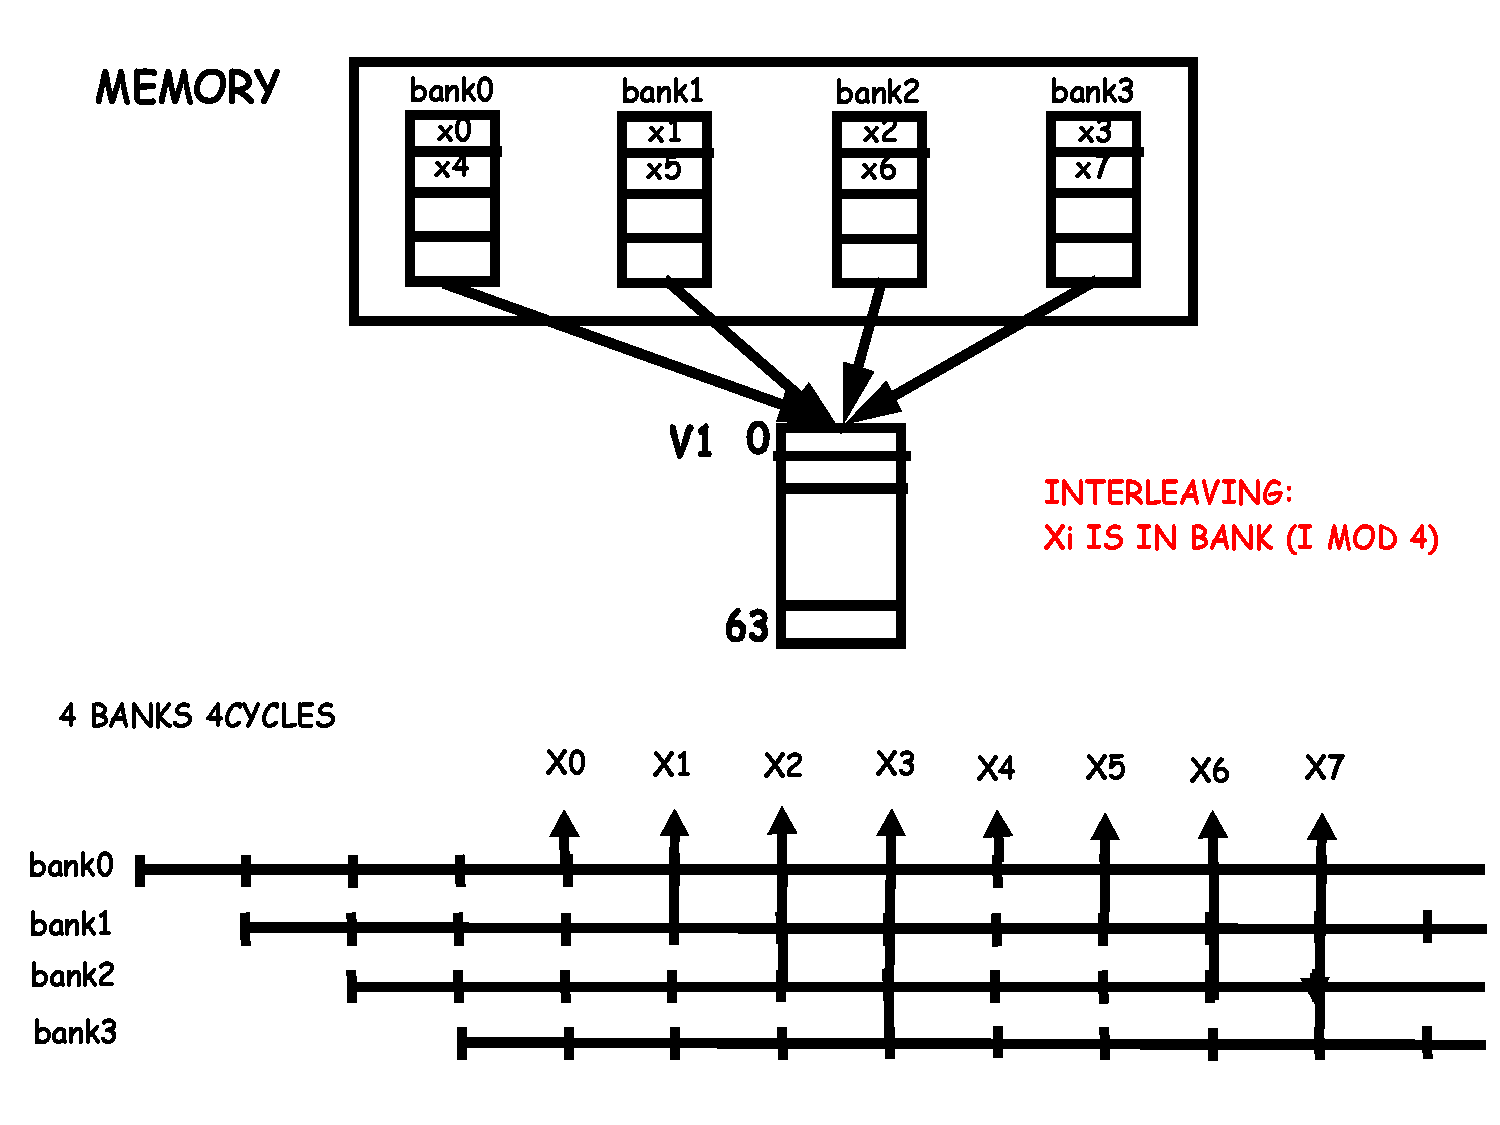
\includegraphics[width=53ex]{Ch1Figs/VectorMemBanksPipe}

\end{frame}

\begin{frame}[fragile,t]
\frametitle{Chaining and Parallel Execution}

\begin{itemize}
    \item Independent Vector Instructions can be executed in parallel
            if functional units are available, but more important\smallskip
    \item They can be chained when there are dependencies. 
            Consider\\ {\tt Y = aX + Y}, where vector length is N:\smallskip

    \item Execution Time (One Vector Op at a time):\\
            {\tt 2*startup(load) + startup(multv) + startup(addv) + 
                    startup(store) + 5*N}\smallskip

    \item Execution Time (Chaining and Parallel):\\
            {\tt startup(load) + startup(addv) + startup(store) + N} 
\end  {itemize}

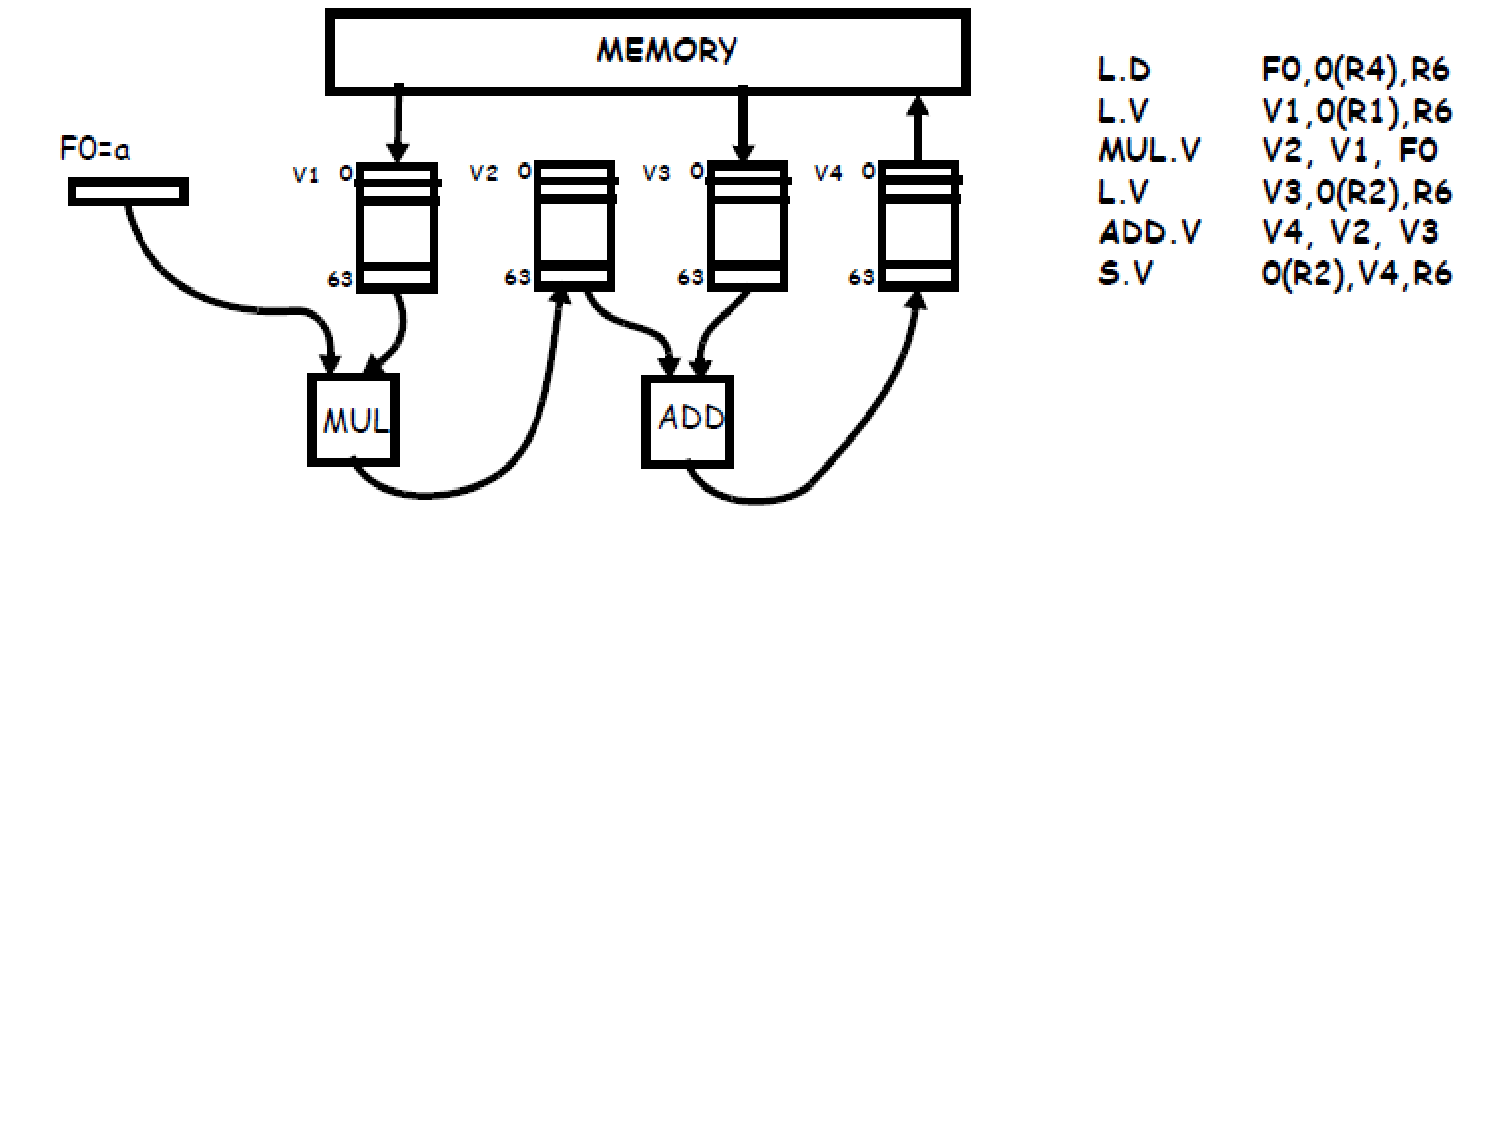
\includegraphics[width=59ex]{Ch1Figs/VectChaining}

\end{frame}

\begin{frame}[fragile,t]
\frametitle{Control Flow \& Indirect Accesses}


For conditional statement use Predicated Instructions
\begin{block}{Fortran Code{\tt~~~~~~~~}Machine Code with Predicated Instructions}
\begin{columns}
\column{0.3\textwidth}
\begin{colorcode}[fontsize=\scriptsize]
DO i = 1, 64, 1
  IF (A(i) .NE. 0) THEN
    A(i) = A(i) - B(i)
  ENDIF
ENDDO
\end{colorcode} 
\column{0.65\textwidth}
\begin{colorcode}[fontsize=\scriptsize]
// Use a Bit-Vector Mask Register VM:
// Assuming A is in V1 and 0 in F0
SNEVS V1, F0   //sets VM(i) if V1(i) \mymath{\neq}F0
SUB.V V1,V1,V2 //subtract under Vector Mask
\end{colorcode}
\end{columns}
\end{block}
\bigskip

Scatter/Gather Operations:
\begin{itemize}
    \item Many scientific computations use sparse matrices\smallskip
    \item Most components are zeros, but under irregular pattern\smallskip

    \item Compress a sparse vector {\tt A} into vectors of non-zero elements:\\
            {\tt A[1:1000] $\Rightarrow$ A$^*$[1:9], K[1:9]},
            where {\tt A$^*$} are the non-zero elements of {\tt A}
            and {\tt K} holds their original indexes. Code example:\smallskip

    \item {\tt DO i = 1, N}\\
            {\tt ~~A(K(i)) = A(K(i)) + C(M(i))}\\
            {\tt ENDDO}
\end  {itemize}

\end{frame}

\begin{frame}[fragile,t]
\frametitle{Memory Scatter/Gather Operations}

\begin{itemize}
    \item Memory Locations of Vector Components are spread out in memory
    \item $\Rightarrow$ use scatter and gather instructions\medskip 
        \begin{itemize}
            \item \emp{\bf Gather} is an instruction loading a set of
                    indirect-indexed addresses into consecutive 
                    vector-register locations\smallskip
            \item \emp{\bf Scatter} is a store instruction from a vector
                    register to indirectly indexed addresses.
        \end  {itemize}
\end  {itemize}

\begin{colorcode}[fontsize=\scriptsize]
L.V   Vk,0(R1),R6  //loads vector K in Register Vk
LI.V  Va,Vk,0(R2)  //gather: loads A(K(i)) into Va
SI.V  Vb,0(R2),Vk  //scatter: stores A(K(i))
\end{colorcode}


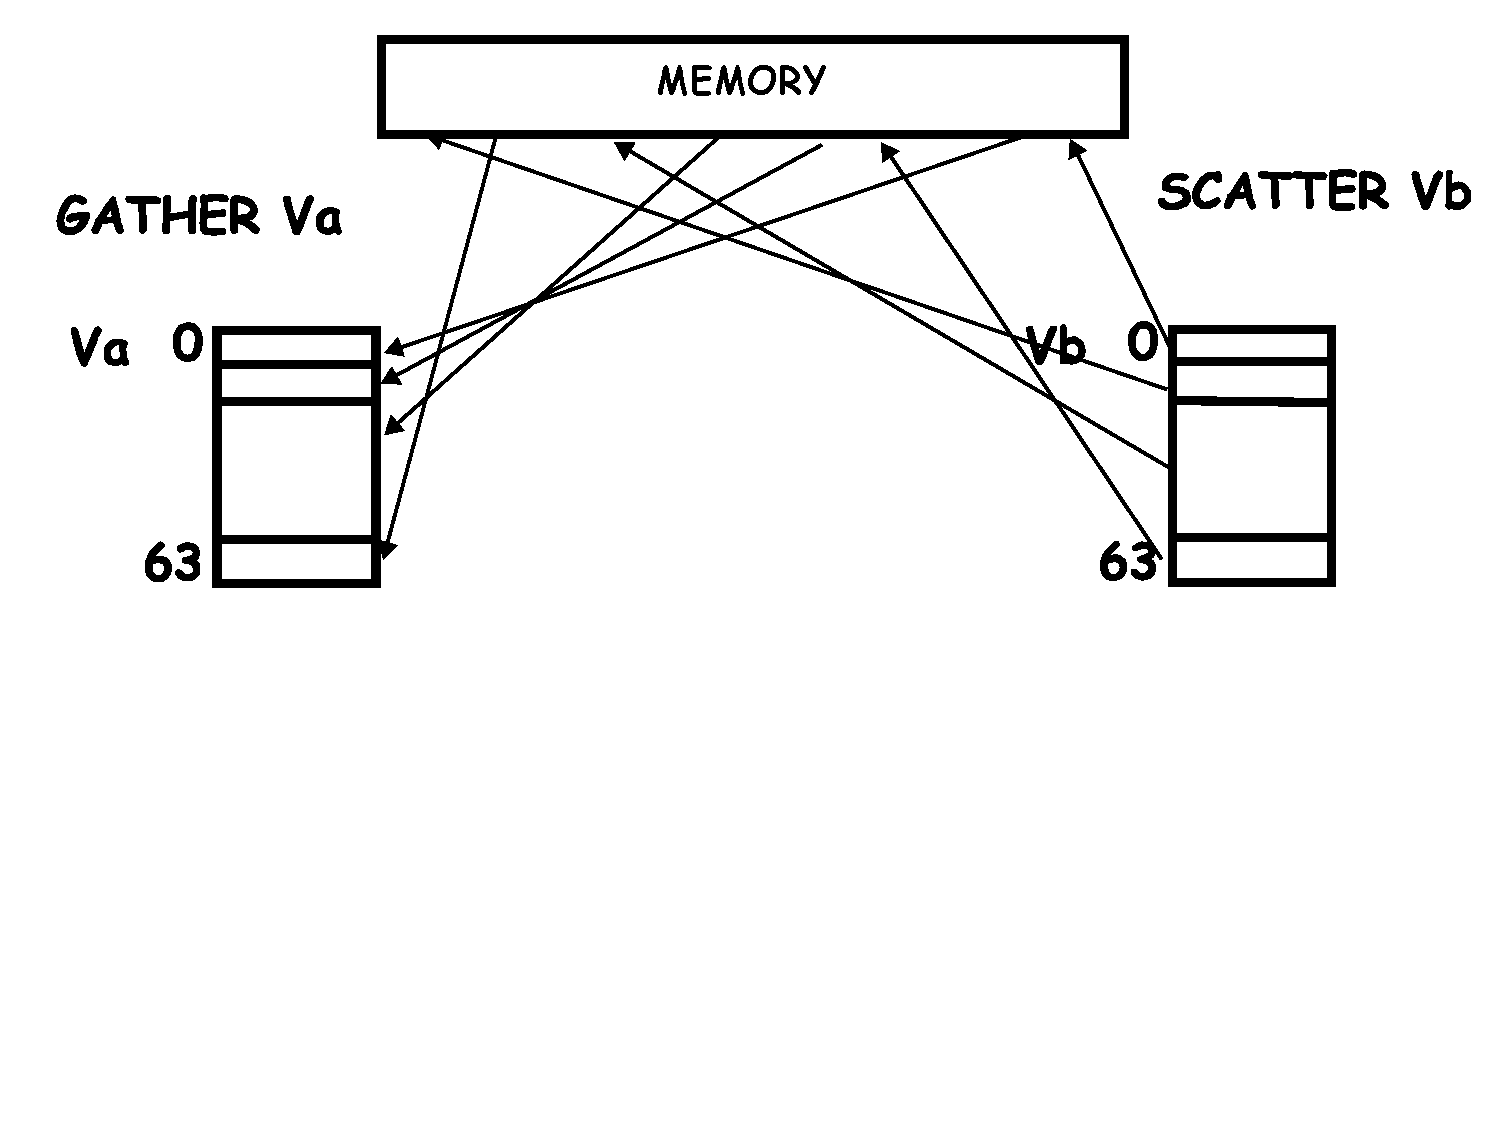
\includegraphics[width=49ex]{Ch1Figs/VectScatterGather}

\end{frame}


\end{document}
